\documentclass[12pt]{article}
\usepackage[utf8]{inputenc}
\usepackage[T1]{fontenc}
\usepackage{geometry}
\usepackage{graphicx}
\usepackage{makeidx}
\geometry{margin=2.5cm}
\usepackage{fancyhdr}

\begin{document}
	
	\thispagestyle{empty}
	
	\begin{center}
		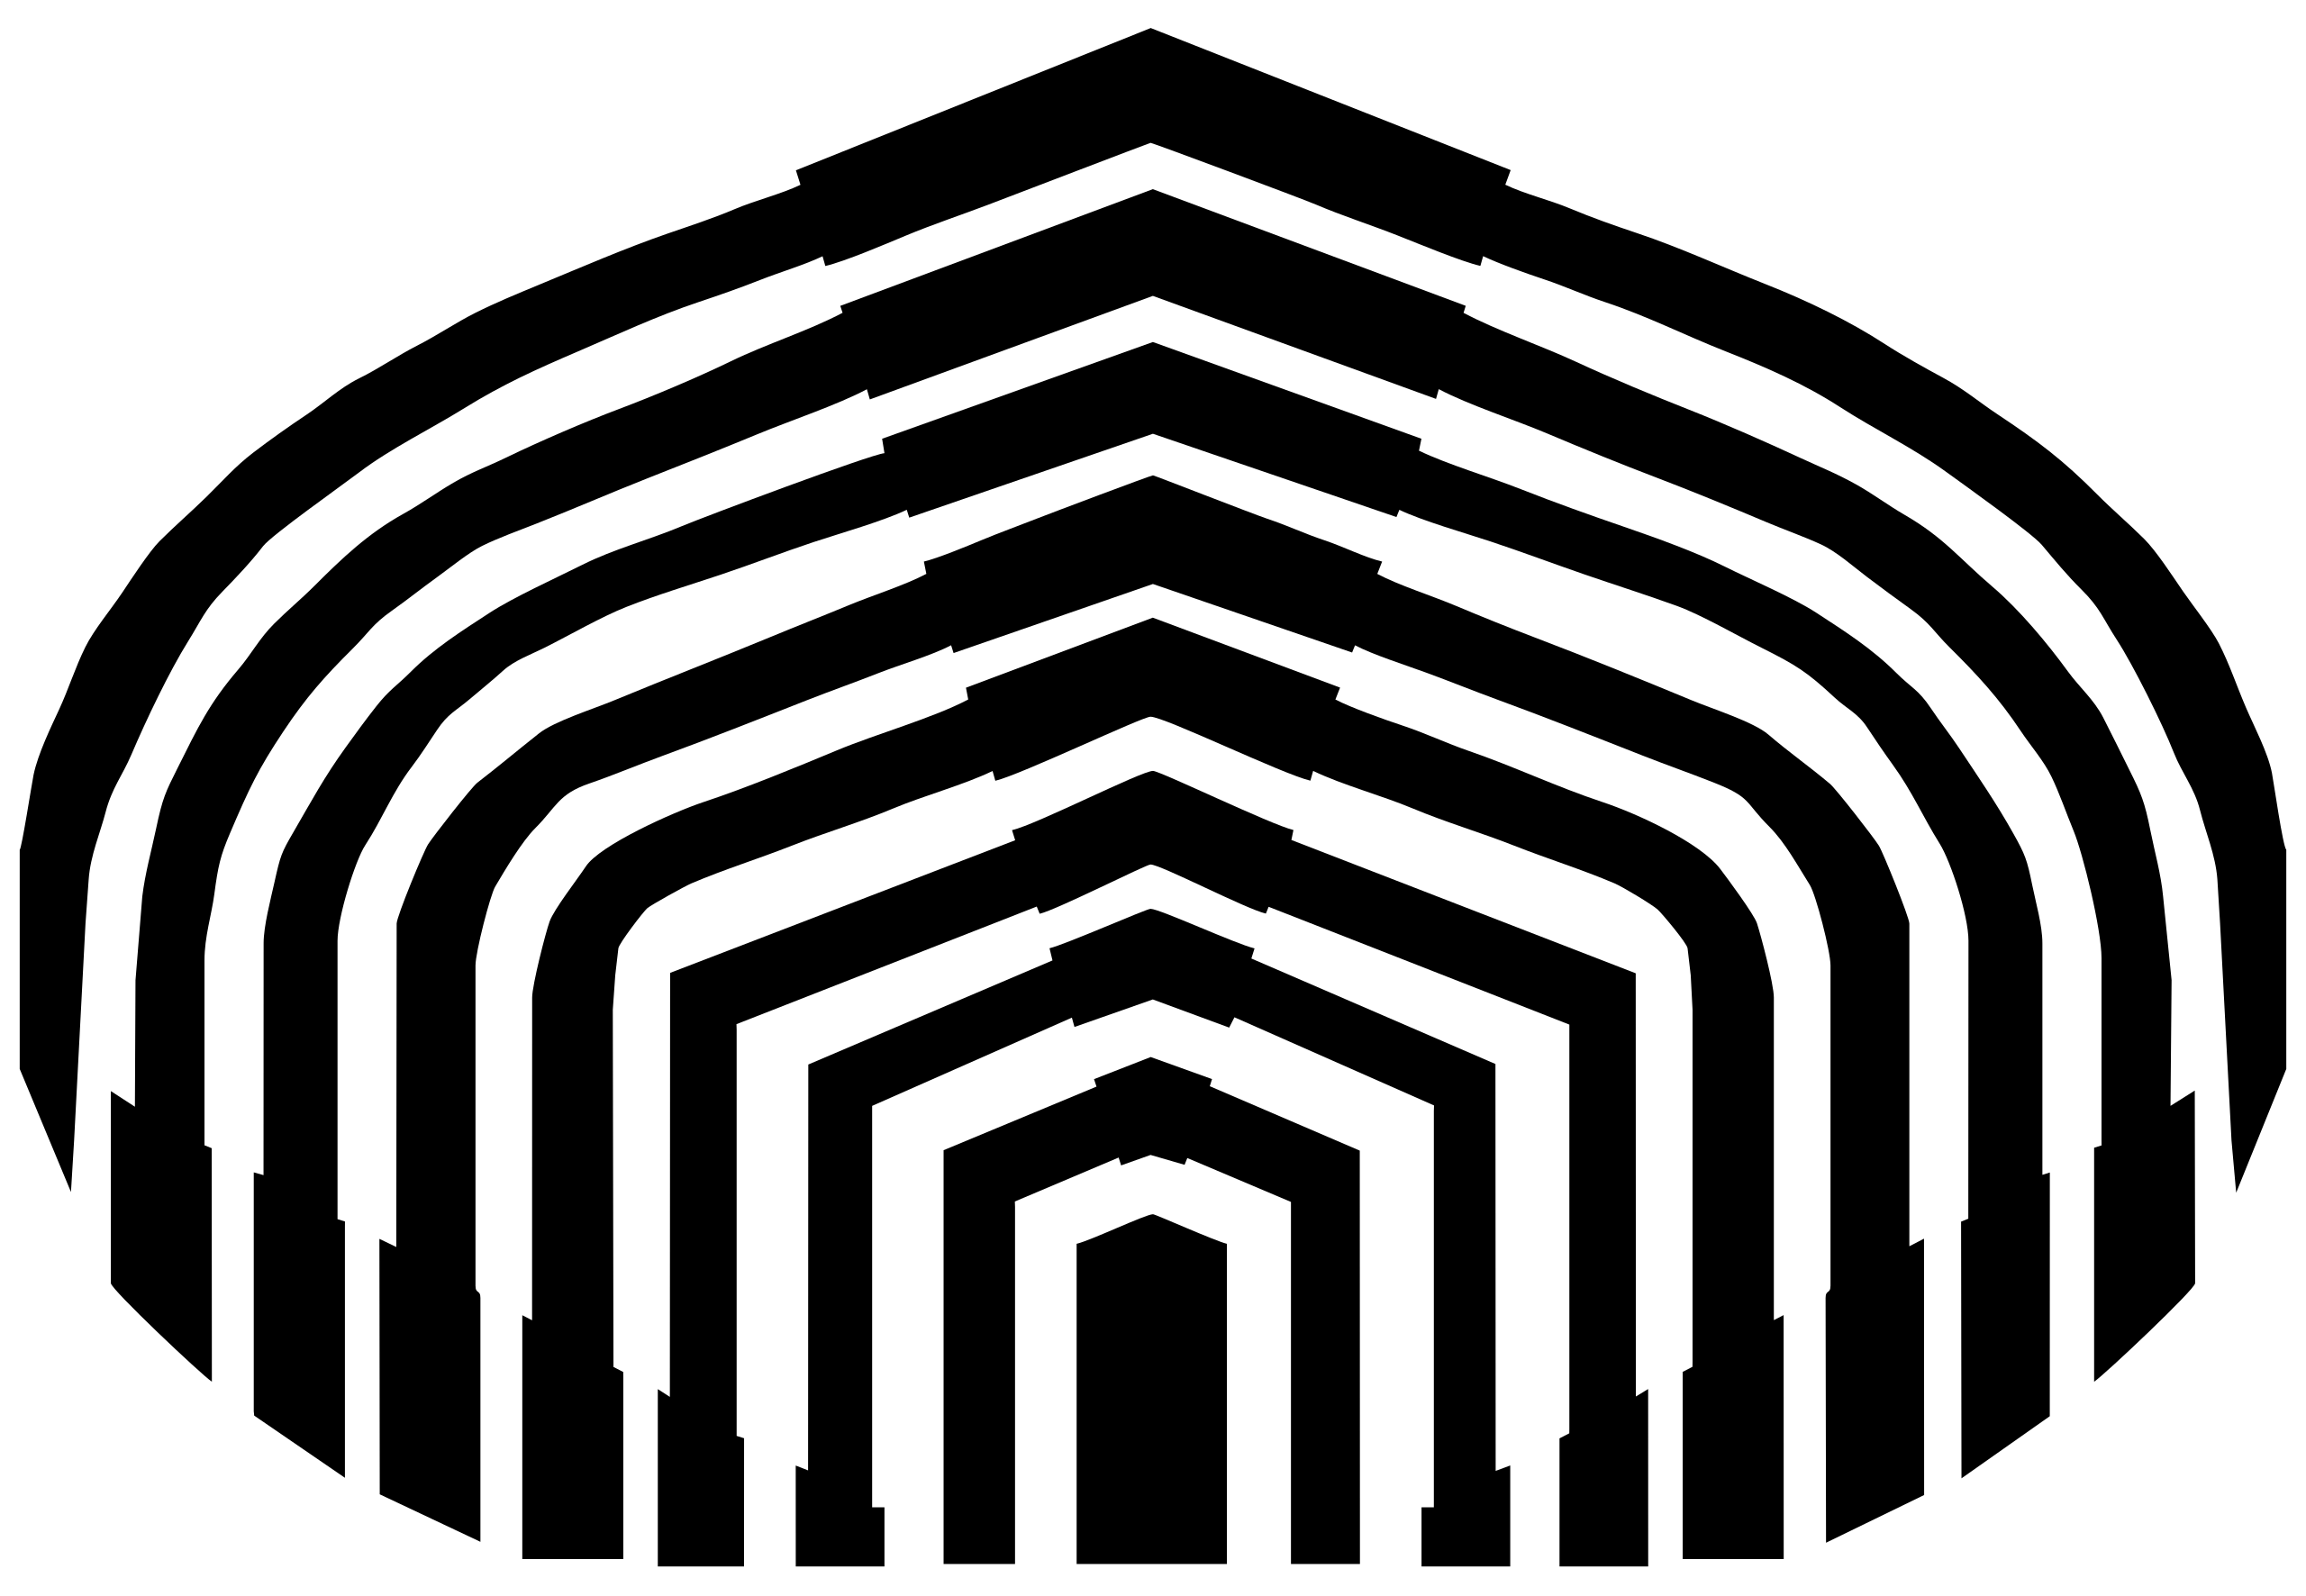
\includegraphics[width=3.1cm,height=2cm]{logo}\\
		UNIVERSIDAD SIMÓN BOLÍVAR\\
		DEPARTAMENTO DE ELECTRÓNICA Y CIRCUITOS\\
		EC1281 - LABORATORIO DE MEDICIONES ELÉCTRICAS\\
		SECCIÓN 1 - GRUPO 1\\
		
		\vspace{7cm}
		\textbf{\Large INFORME - PRÁCTICA \#4}\\
		EL OSCILOSCOPIO\\
	\end{center}
	
	\begin{flushleft}
		\vspace{9cm}
		\hfill Integrantes:\\
		\hfill {\large Luis Becerra - 1910557}\\
		\hfill {\large Lorena Rojas - 1910469}\\
	\end{flushleft}
	
	\newpage
	
	\pagenumbering{Roman}
        \setcounter{page}{2}
	
	\begin{center}
		\textbf{\large RESUMEN}\\
	\end{center}
	
        El objetivo de este informe de laboratorio de mediciones eléctricas fue analizar el funcionamiento y las características del osciloscopio como herramienta fundamental en el estudio de señales eléctricas. Para ello, se siguió un procedimiento que incluyó la configuración adecuada del osciloscopio, la medición de diferentes señales y la interpretación de los resultados obtenidos. Los resultados más relevantes revelaron la capacidad del osciloscopio para mostrar con precisión la forma de onda de las señales, así como la medición de su frecuencia, amplitud y tiempo. Además, se destacó la utilidad de las diferentes funciones y ajustes disponibles en el osciloscopio. Como conclusión fundamental, se evidenció la importancia del osciloscopio como herramienta indispensable en el análisis y diagnóstico de circuitos eléctricos, ya que permite visualizar y medir de manera precisa las señales eléctricas. En resumen, este informe de laboratorio proporciona una visión clara y concisa del objetivo, procedimiento, resultados y conclusiones relacionados con el estudio del osciloscopio en mediciones eléctricas.\\
	
	\newpage
	
	\begin{center}
		\textbf{\large ÍNDICE}\\
	\end{center}
	
	\noindent \textbf{RESUMEN} \hfill \textbf{II}\\
	\noindent \textbf{ÍNDICE} \hfill \textbf{III}\\
	\noindent \textbf{MARCO TEÓRICO} \hfill \textbf{1}\\
	\noindent \textbf{METEDOLOGÍA} \hfill \textbf{3}\\
	\noindent \textbf{RESULTADOS} \hfill \textbf{4}\\
	\noindent \textbf{ANÁLISIS DE RESULTADOS} \hfill \textbf{11}\\
	\noindent \textbf{CONCLUSIONES} \hfill \textbf{14}\\
	\noindent \textbf{BIBLIOGRAFÍA} \hfill \textbf{17}\\
	
	\newpage
	
	\pagenumbering{arabic}
	
	\begin{center}
		\textbf{\large MARCO TEÓRICO}\\
	\end{center}
	
	\textbf{1. Osciloscopio Analógico:}

        \begin{itemize}
            \item Los osciloscopios analógicos utilizan tubos de rayos catódicos (TRC) para mostrar las señales en una pantalla de fósforo. Proporcionan una representación visual continua y suave de las señales eléctricas.
            \item Son adecuados para la observación de señales de alta frecuencia y muestran la amplitud y la forma de onda de manera precisa.
            \item Tienen una respuesta en tiempo real, lo que significa que las señales se muestran instantáneamente sin demoras.
            \item La velocidad de actualización de la pantalla en los osciloscopios analógicos es rápida y permite una visualización en tiempo real de las señales.
            \item Son menos costosos en comparación con los osciloscopios digitales y son ampliamente utilizados en aplicaciones de audio, radiofrecuencia y señales analógicas en general.
        \end{itemize}
        
        \textbf{2. Osciloscopio Digital:}

        \begin{itemize}
            \item Los osciloscopios digitales capturan las señales y las convierten en datos digitales para su visualización en una pantalla LCD. Proporcionan mediciones más precisas y una mayor funcionalidad en comparación con los osciloscopios analógicos.
            \item Tienen una mayor resolución y precisión en la medición de amplitud, frecuencia, tiempo y otras características de las señales.
            \item Ofrecen una amplia gama de funciones adicionales, como almacenamiento y análisis de datos, capacidad de realizar mediciones automáticas, cálculos matemáticos en tiempo real y visualización de múltiples formas de onda en pantalla.
            \item Tienen una alta velocidad de muestreo, lo que permite capturar detalles finos de las señales de alta frecuencia.
            \item La capacidad de almacenamiento permite capturar y analizar señales complejas y realizar comparaciones con señales de referencia.
        \end{itemize}
        
        \textbf{3. Generador de Funciones:}

        \begin{itemize}
            \item El generador de funciones es un dispositivo utilizado para generar señales eléctricas de diferentes formas y frecuencias. Es una herramienta fundamental en pruebas, experimentos y diseño de circuitos electrónicos.
            \item Puede producir señales senoidales, cuadradas, triangulares y de otras formas, con una amplitud y frecuencia ajustables.
            \item Los generadores de funciones también pueden tener funciones adicionales, como la modulación de amplitud y frecuencia, así como la capacidad de barrido de frecuencia.
            \item Permiten simular diferentes condiciones de señal y generar señales de prueba para verificar y calibrar equipos electrónicos.
            \item Son ampliamente utilizados en aplicaciones como comunicaciones, pruebas de respuesta en frecuencia, diseño de circuitos, educación y muchas otras áreas de la electrónica.
        \end{itemize}
        
        En resumen, los osciloscopios analógicos ofrecen una representación visual continua y suave de las señales, son adecuados para señales de alta frecuencia y tienen una respuesta en tiempo real. Los osciloscopios digitales ofrecen mediciones más precisas, funciones adicionales avanzadas y una alta velocidad de muestreo. Por otro lado, los generadores de funciones son dispositivos versátiles que permiten generar señales de diferentes formas y frecuencias para pruebas y diseño de circuitos electrónicos.
        
	\newpage
	
	\begin{center}
		\textbf{\large METODOLOGÍA}\\
	\end{center}

        \textbf{1. Medición de amplitudes:}\\
        
        Para medir las amplitudes de las señales, tanto continuas como alternas, en un osciloscopio digital, se deben seguir los siguientes pasos. Primero, se conecta la punta de prueba al canal correspondiente y se ajusta el factor de multiplicación adecuado (X1 o X10). A continuación, se conecta la punta de prueba al circuito o fuente que se desea medir. Luego, se ajustan los controles de calibración de la escala horizontal y vertical, así como el selector de disparo, para obtener una visualización precisa de la forma de onda. Finalmente, se toman las medidas de amplitud utilizando las escalas proporcionales en el eje vertical del osciloscopio.\\

        \textbf{2. Medición de frecuencias:}\\
        
        Para medir la frecuencia de las señales periódicas en el osciloscopio utilizando la calibración de tiempo del eje horizontal, se siguen los siguientes pasos. Primero, se conecta la señal al canal adecuado y se selecciona dicho canal y su disparo en el osciloscopio. Se coloca la referencia de tierra en el centro de la pantalla y se ajusta la ganancia del canal vertical para visualizar claramente la señal. A continuación, se cuenta el número de divisiones y subdivisiones horizontales entre dos puntos de referencia de la señal (como dos máximos, dos mínimos o dos cruces por cero) y se multiplica este valor por el número indicado en el control de calibración de la escala horizontal. El resultado obtenido es el periodo de la señal, y su inverso corresponde a la frecuencia.\\

        \textbf{3. Medición del desfasaje:}\\
        
        Para medir el desfase entre dos señales cuando ambas están referidas a la tierra del circuito (como el voltaje de la fuente Vg y el voltaje en el condensador VC), se siguen los siguientes pasos. Se conectan las señales a los canales verticales correspondientes del osciloscopio, asegurándose de que tengan la misma frecuencia. Luego, se ajusta el control de calibración de la escala horizontal para visualizar uno o dos ciclos completos de las señales. Se selecciona el acoplamiento de señal en GND para cada canal vertical y se ajusta la posición vertical para que las líneas de 0V de ambos canales se ubiquen en el centro de la pantalla. A continuación, se cambia el acoplamiento de señal a AC en ambos canales. Se cuenta el número de divisiones horizontales correspondientes a un ciclo completo de la sinusoide (periodo T) y se toma nota de este valor. Luego, se cuenta el número de divisiones entre un punto específico de una señal y un punto de la otra señal que tenga la misma fase. Finalmente, se utiliza una regla de tres para determinar el desfase entre las señales, teniendo en cuenta que un ciclo completo corresponde a un desfase de $2\pi$ radianes o 360 grados. Es importante considerar las conexiones a tierra adecuadas para evitar errores en las mediciones.
	
	\newpage
	
	\begin{center}
		\textbf{\large RESULTADOS}\\
	\end{center}
	
	\noindent En el laboratorio se midió lo siguiente:
	
	\begin{center}
		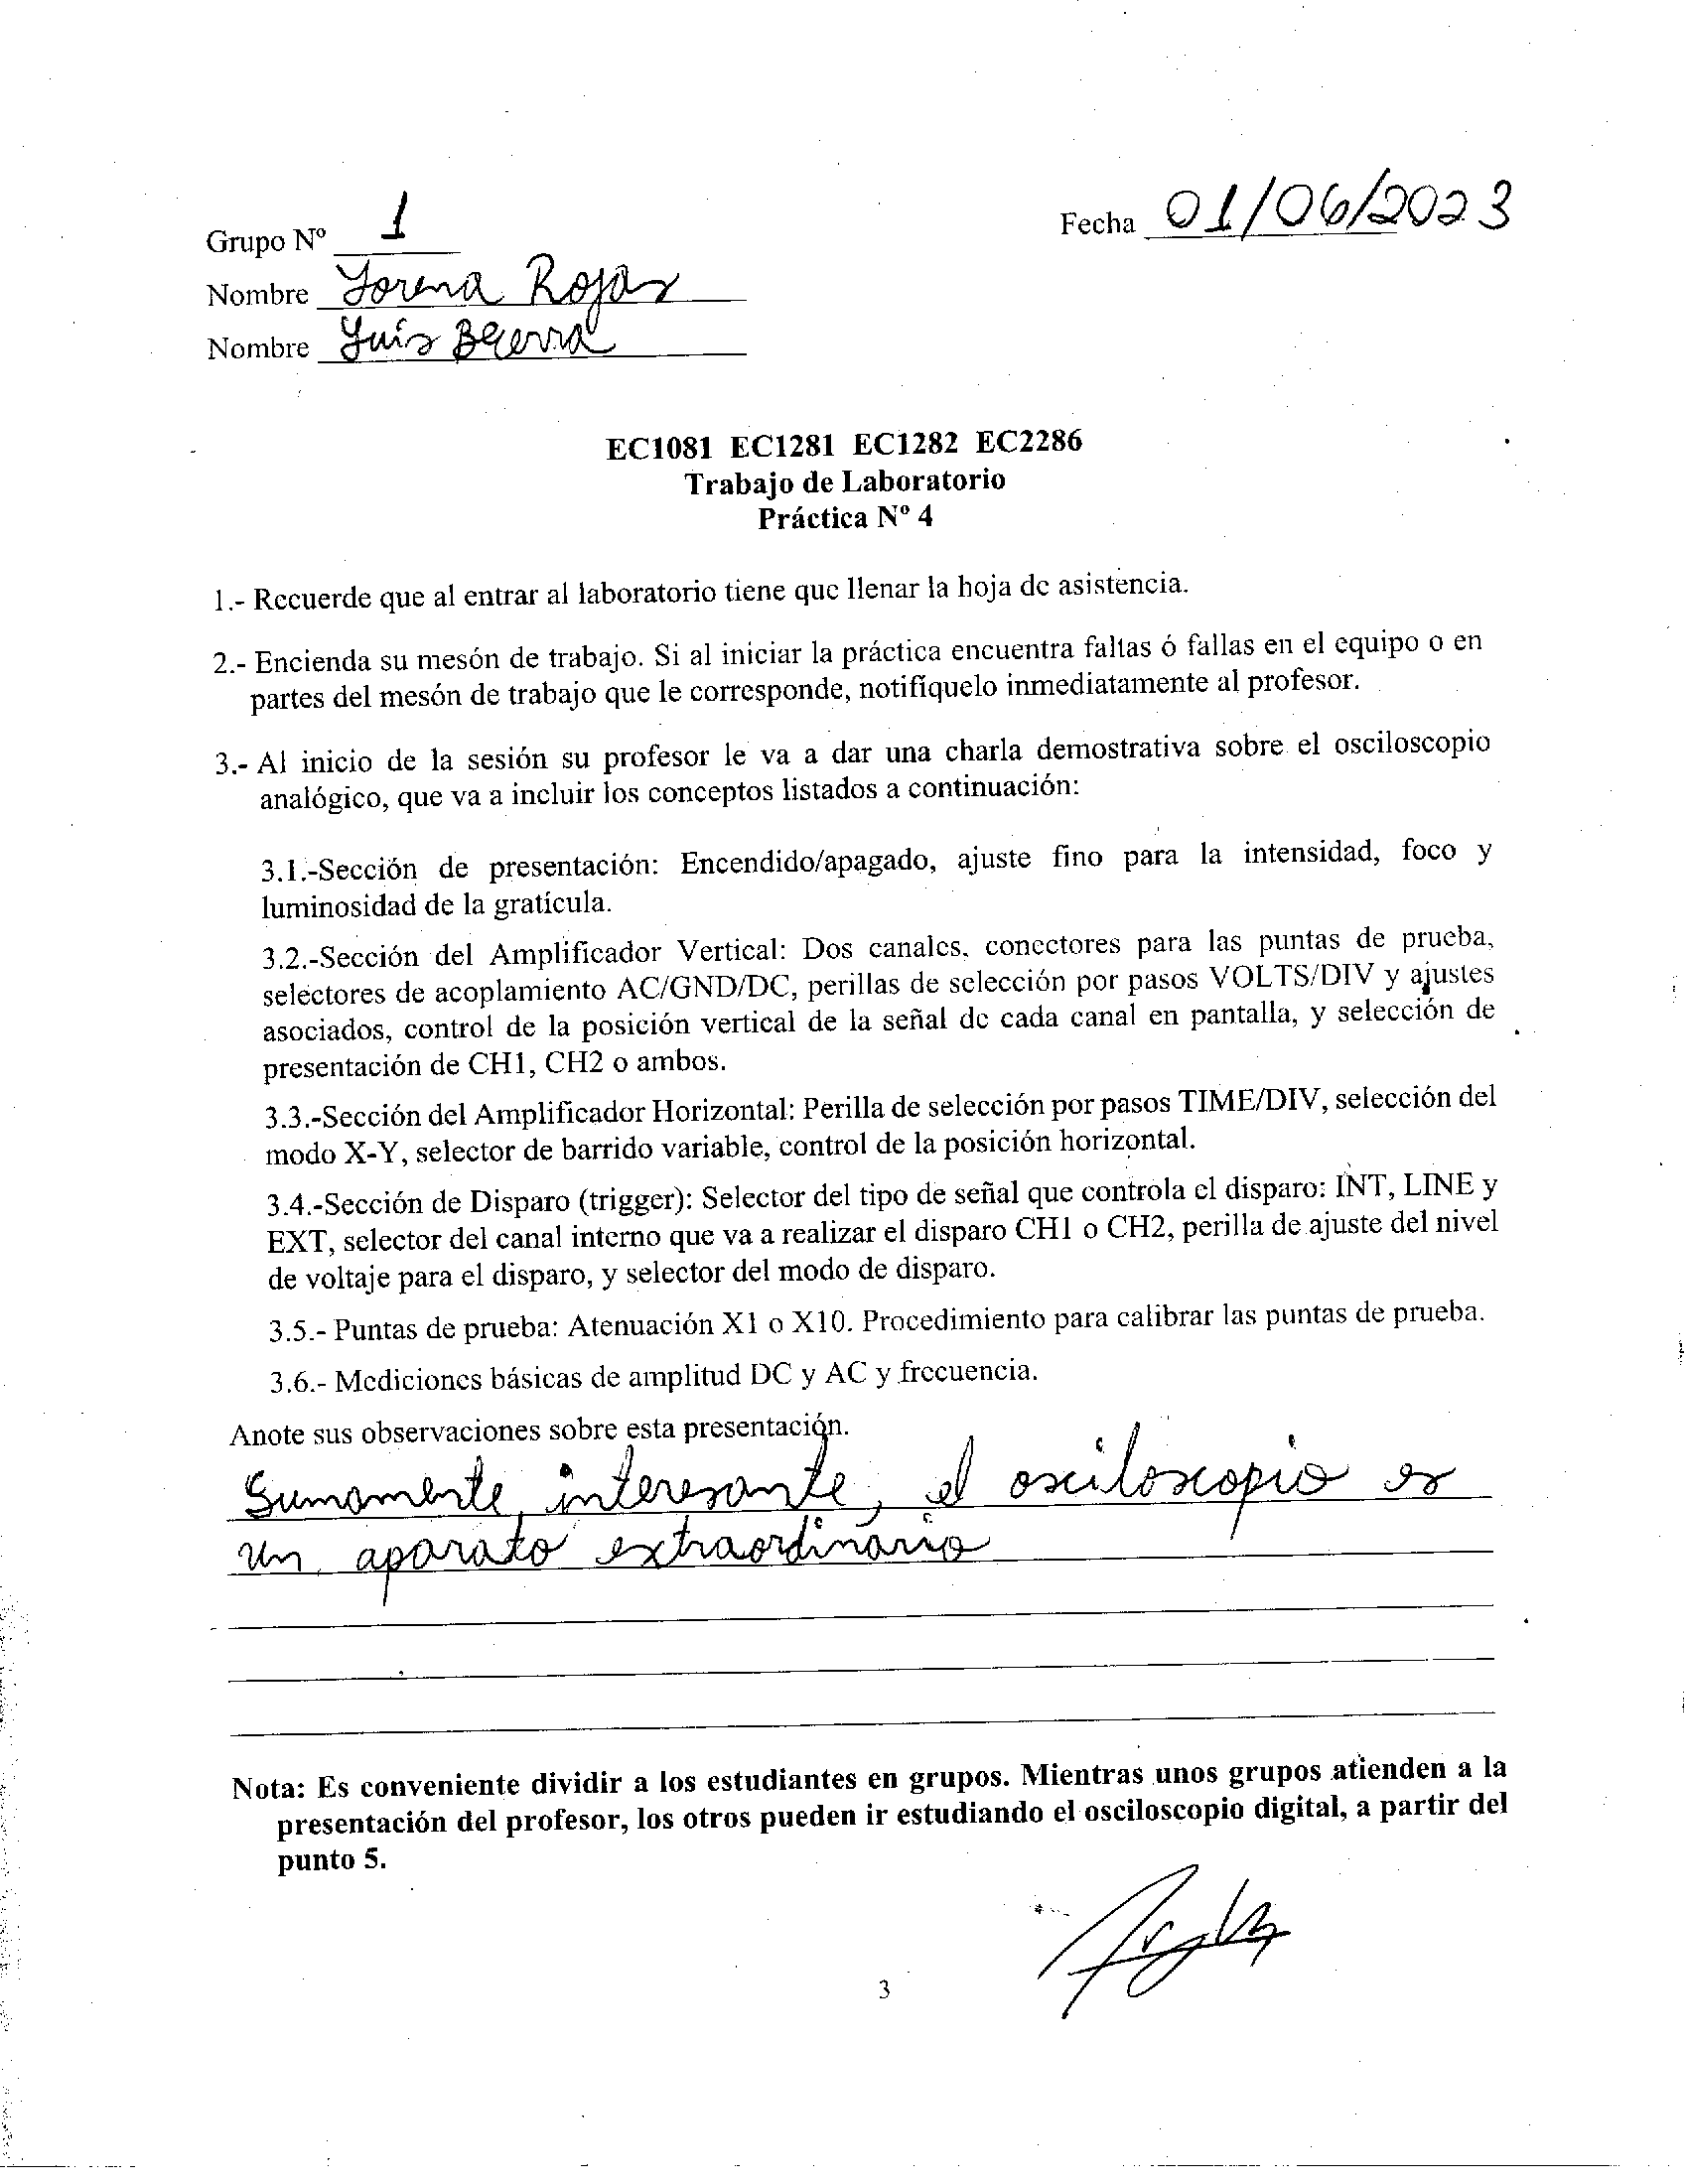
\includegraphics[width=16cm,height=20cm]{Img/anex_lab_4_0001}
	\end{center}
	
	\begin{center}
		\includegraphics[width=16cm,height=20cm]{Img/anex_lab_4_0002}
	\end{center}
	
	\begin{center}
		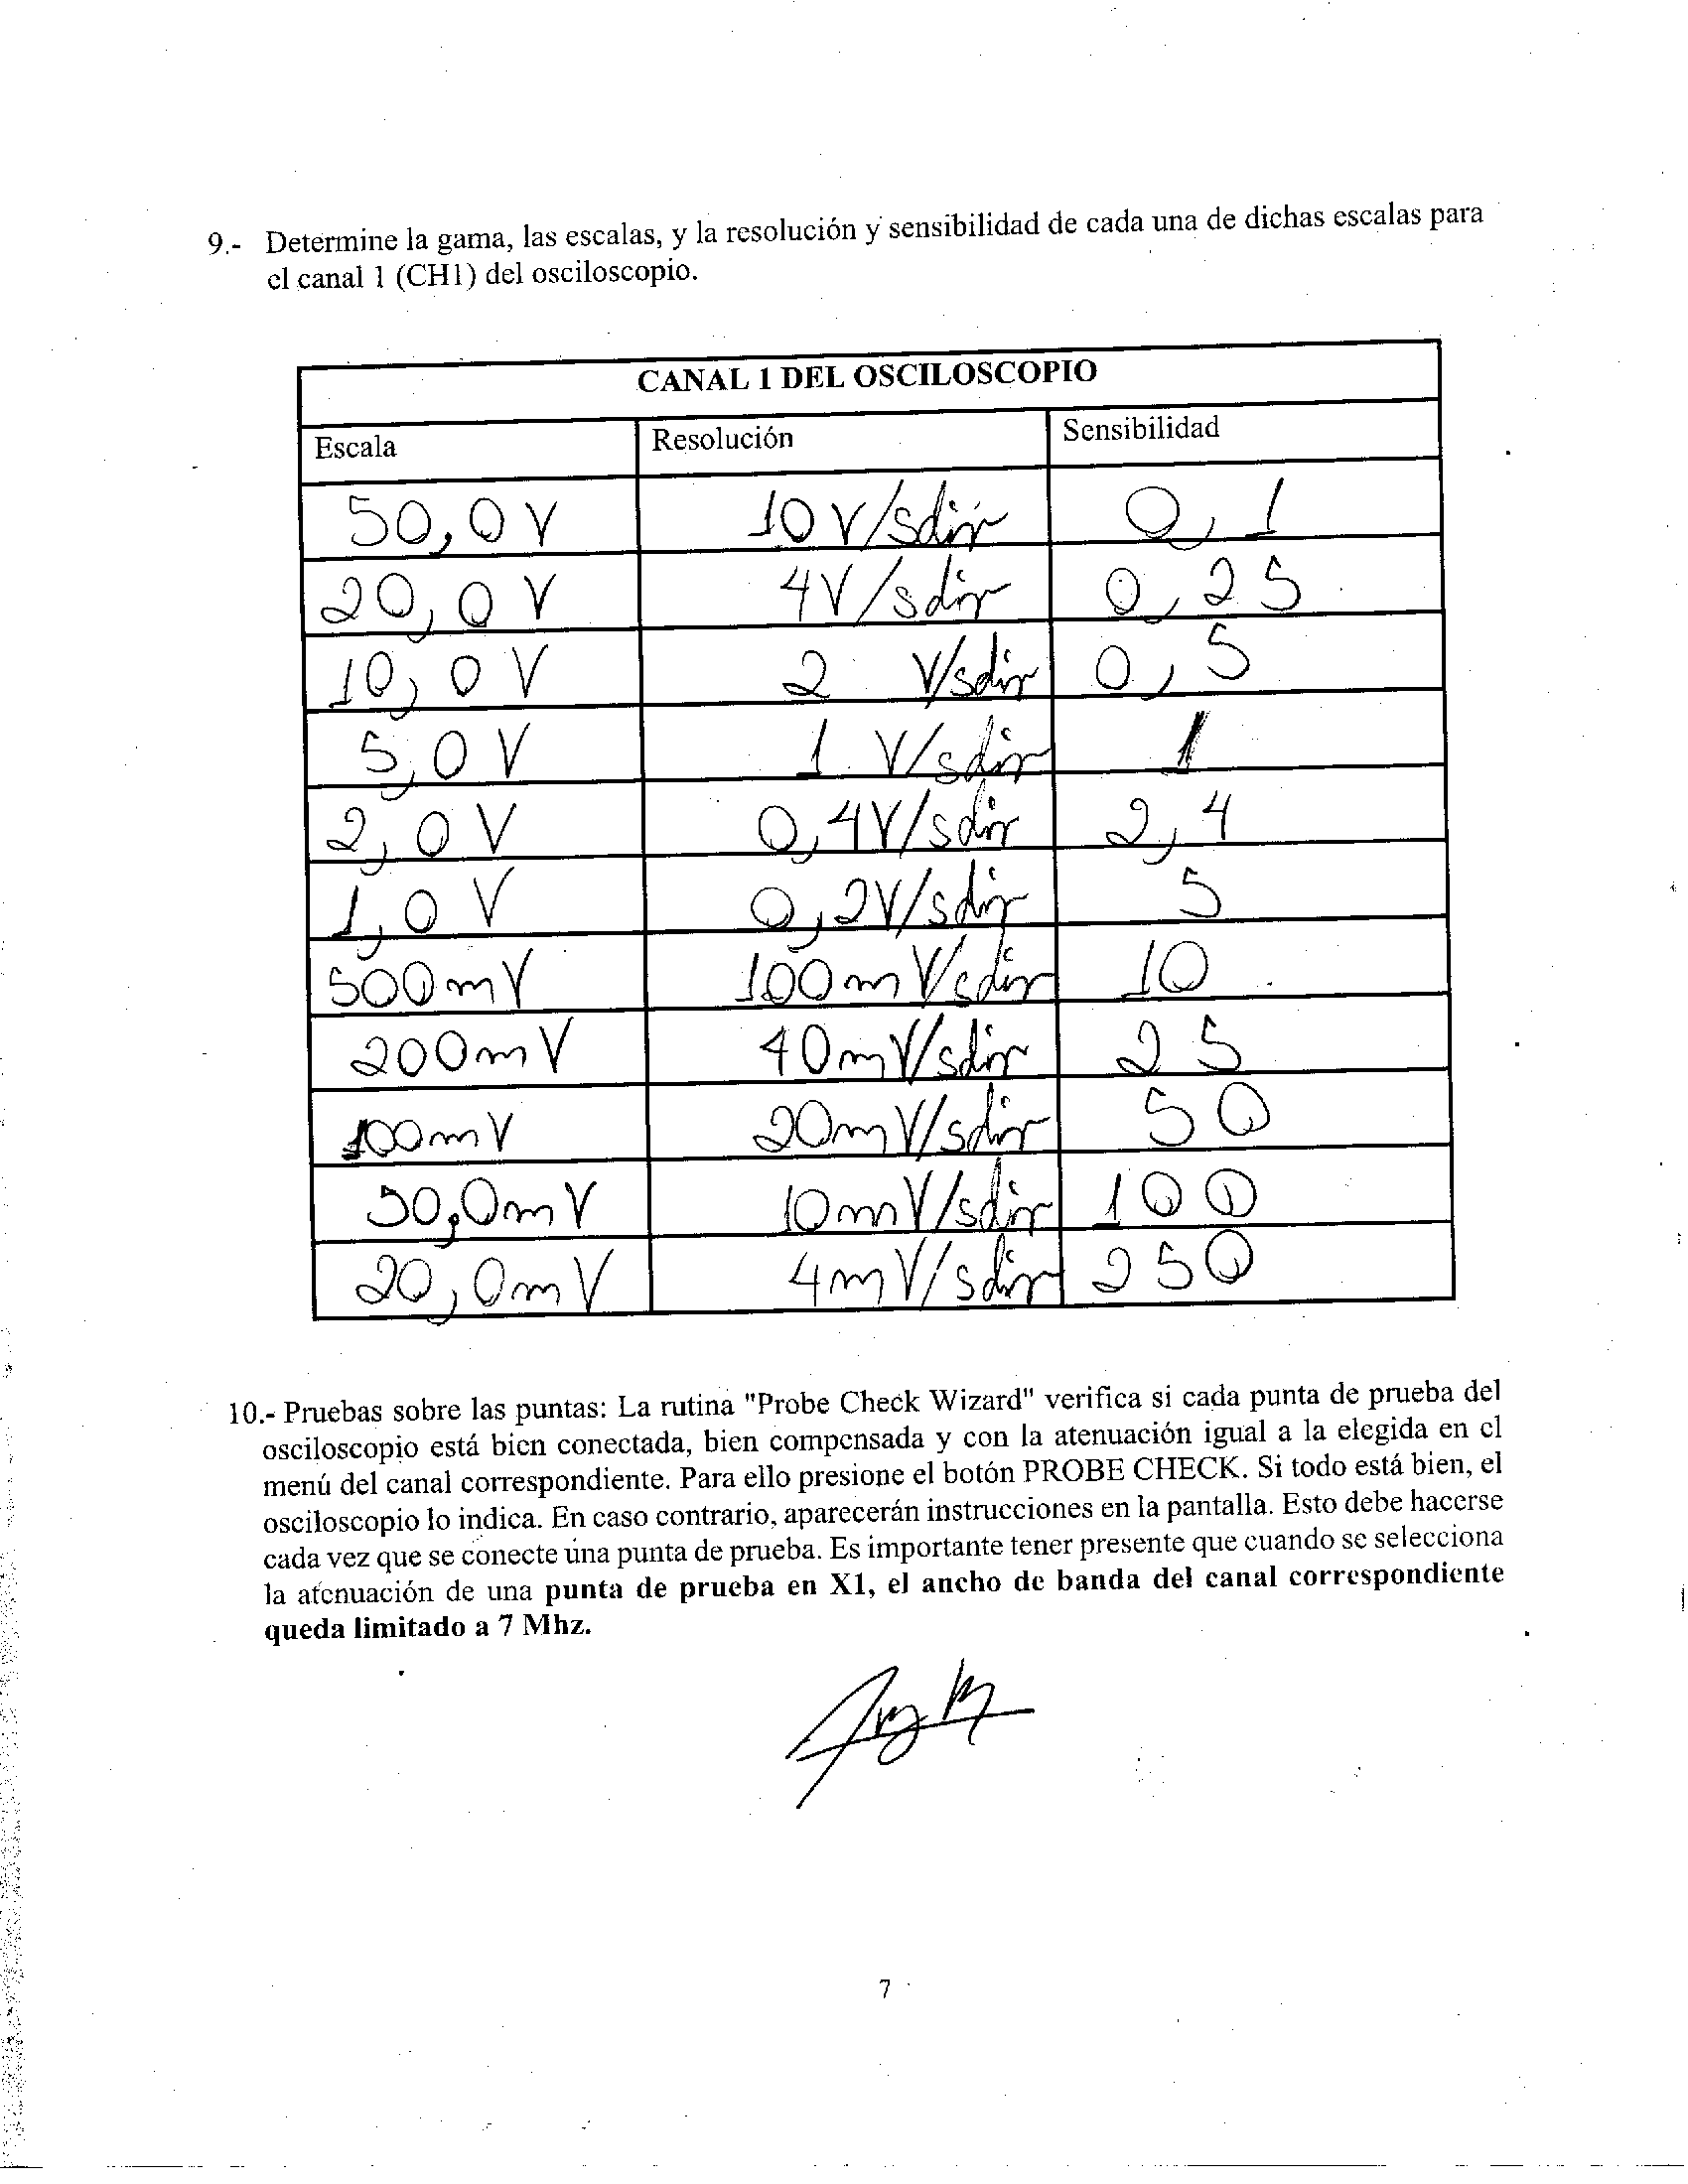
\includegraphics[width=16cm,height=20cm]{Img/anex_lab_4_0003}
	\end{center}
	
	\begin{center}
		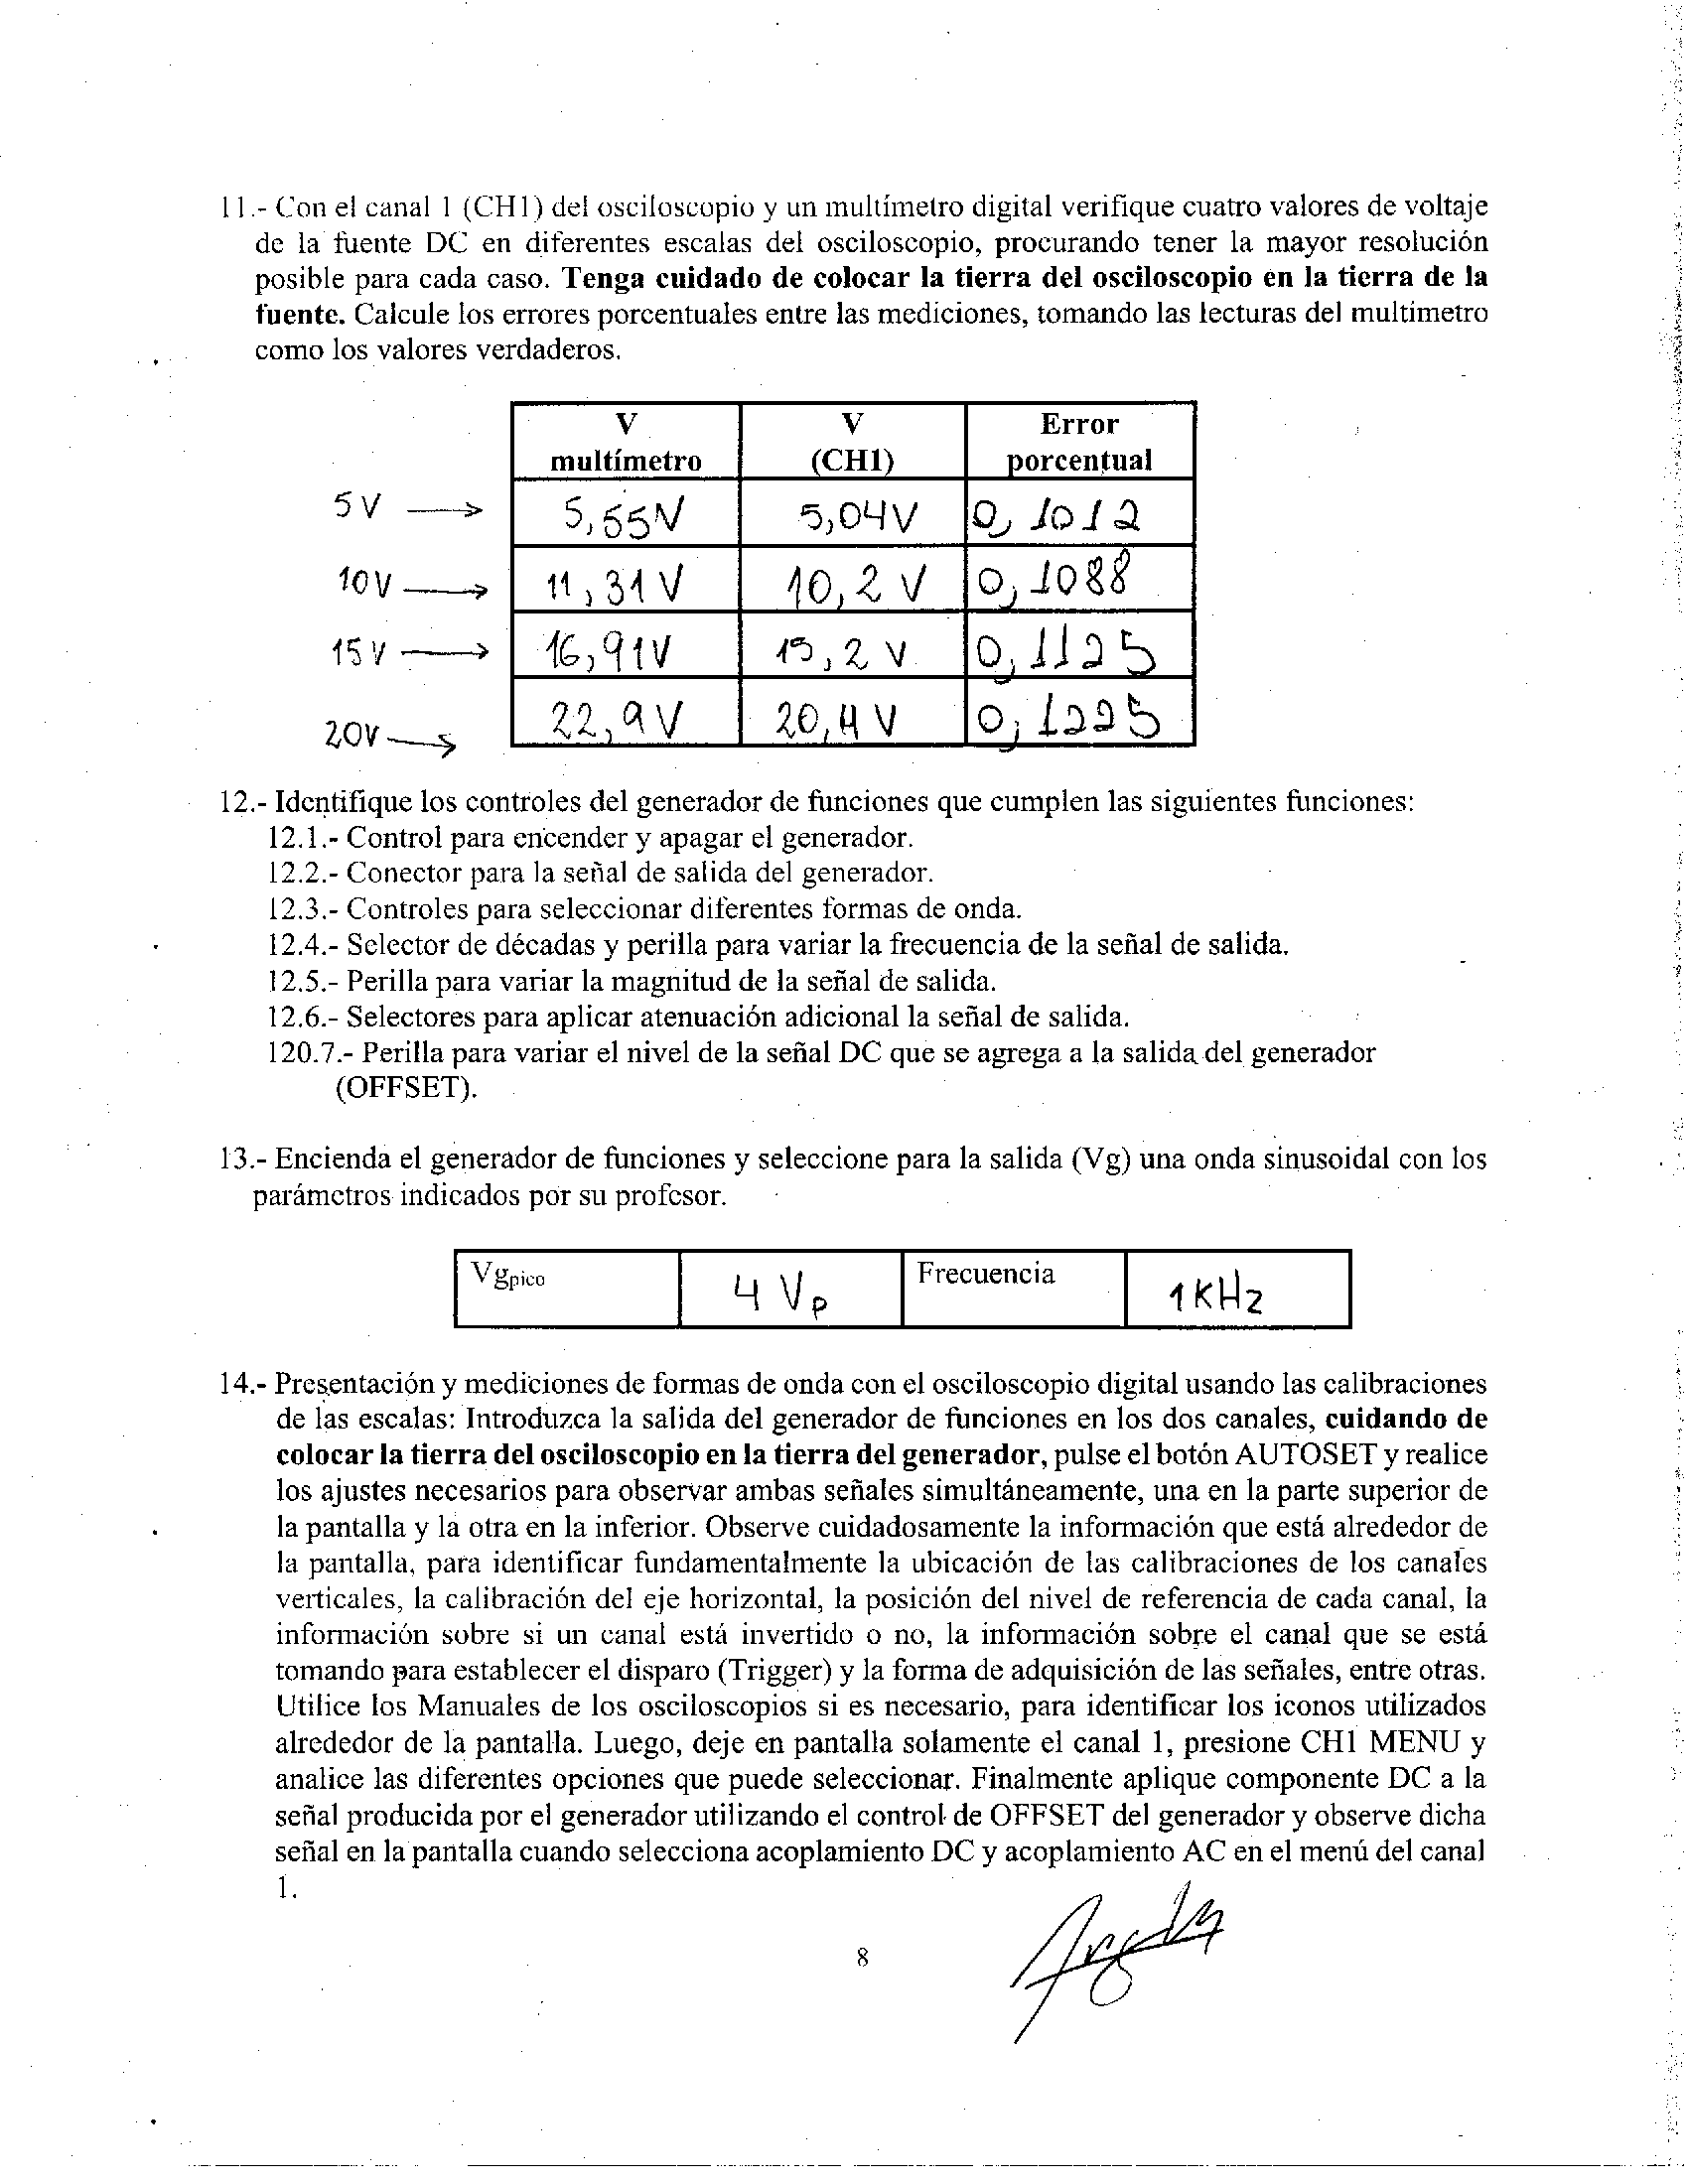
\includegraphics[width=16cm,height=20cm]{Img/anex_lab_4_0004}
	\end{center}
	
	\begin{center}
		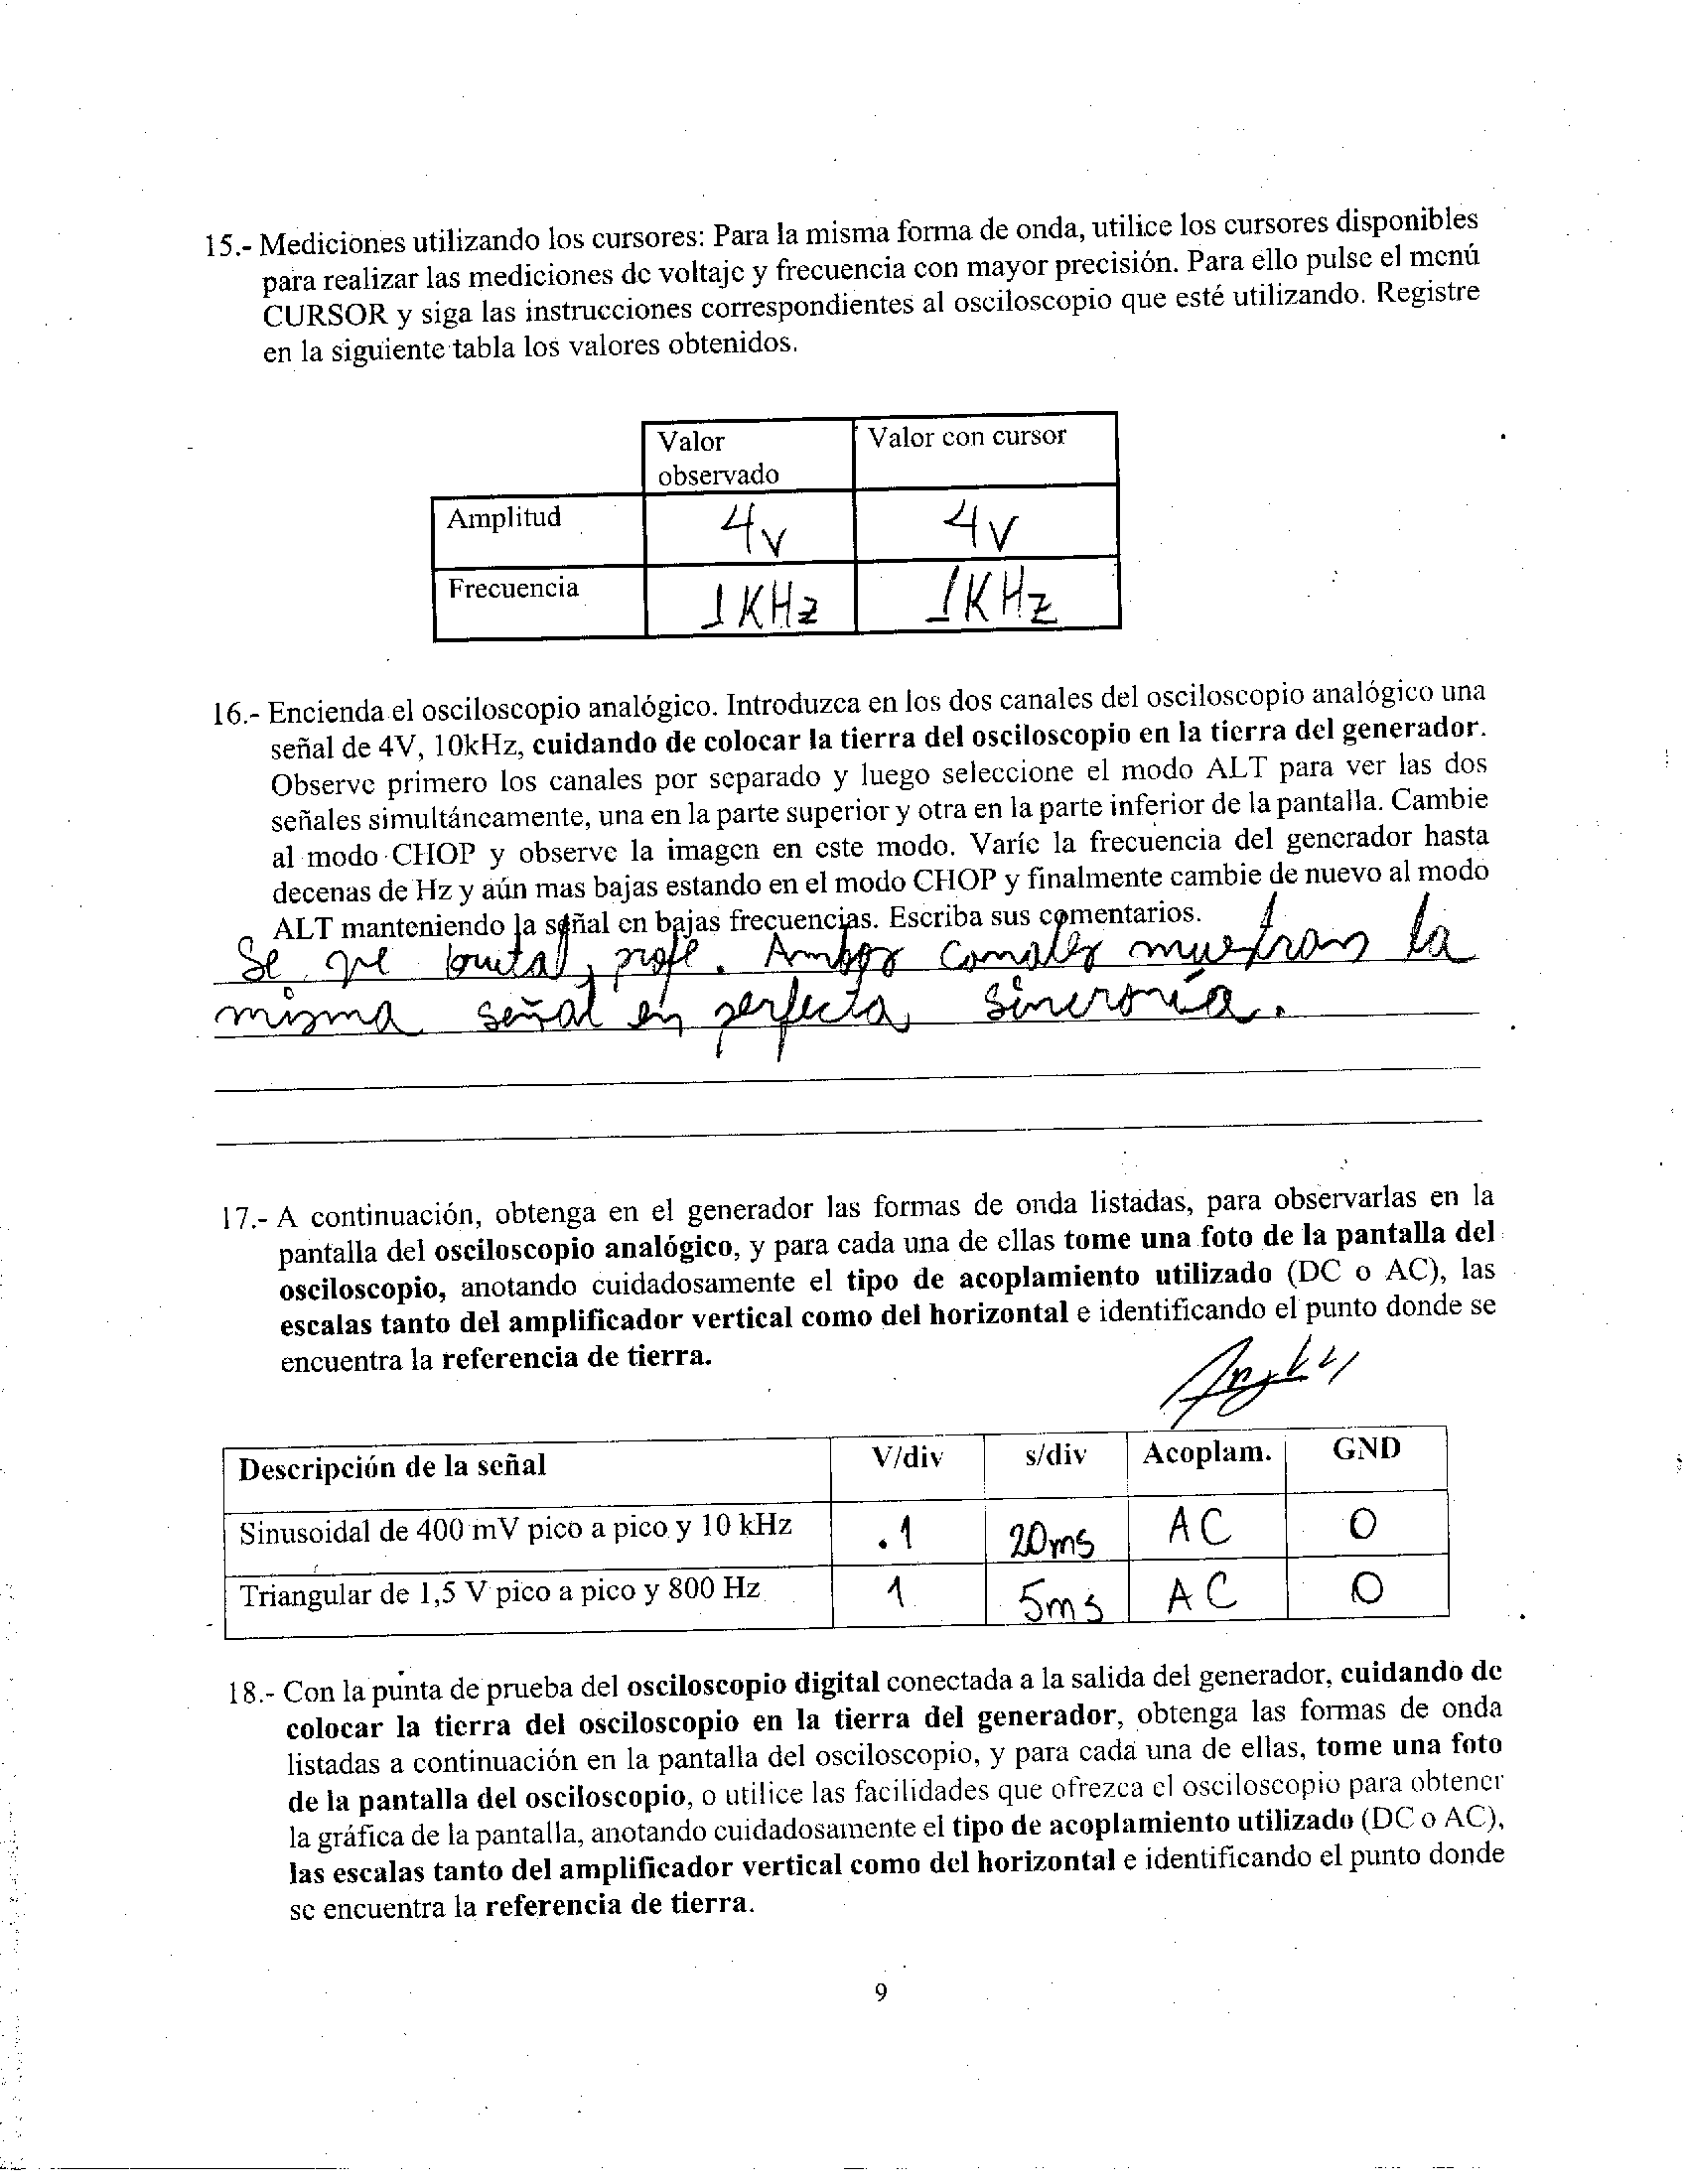
\includegraphics[width=16cm,height=20cm]{Img/anex_lab_4_0005}
	\end{center}
	
	\begin{center}
		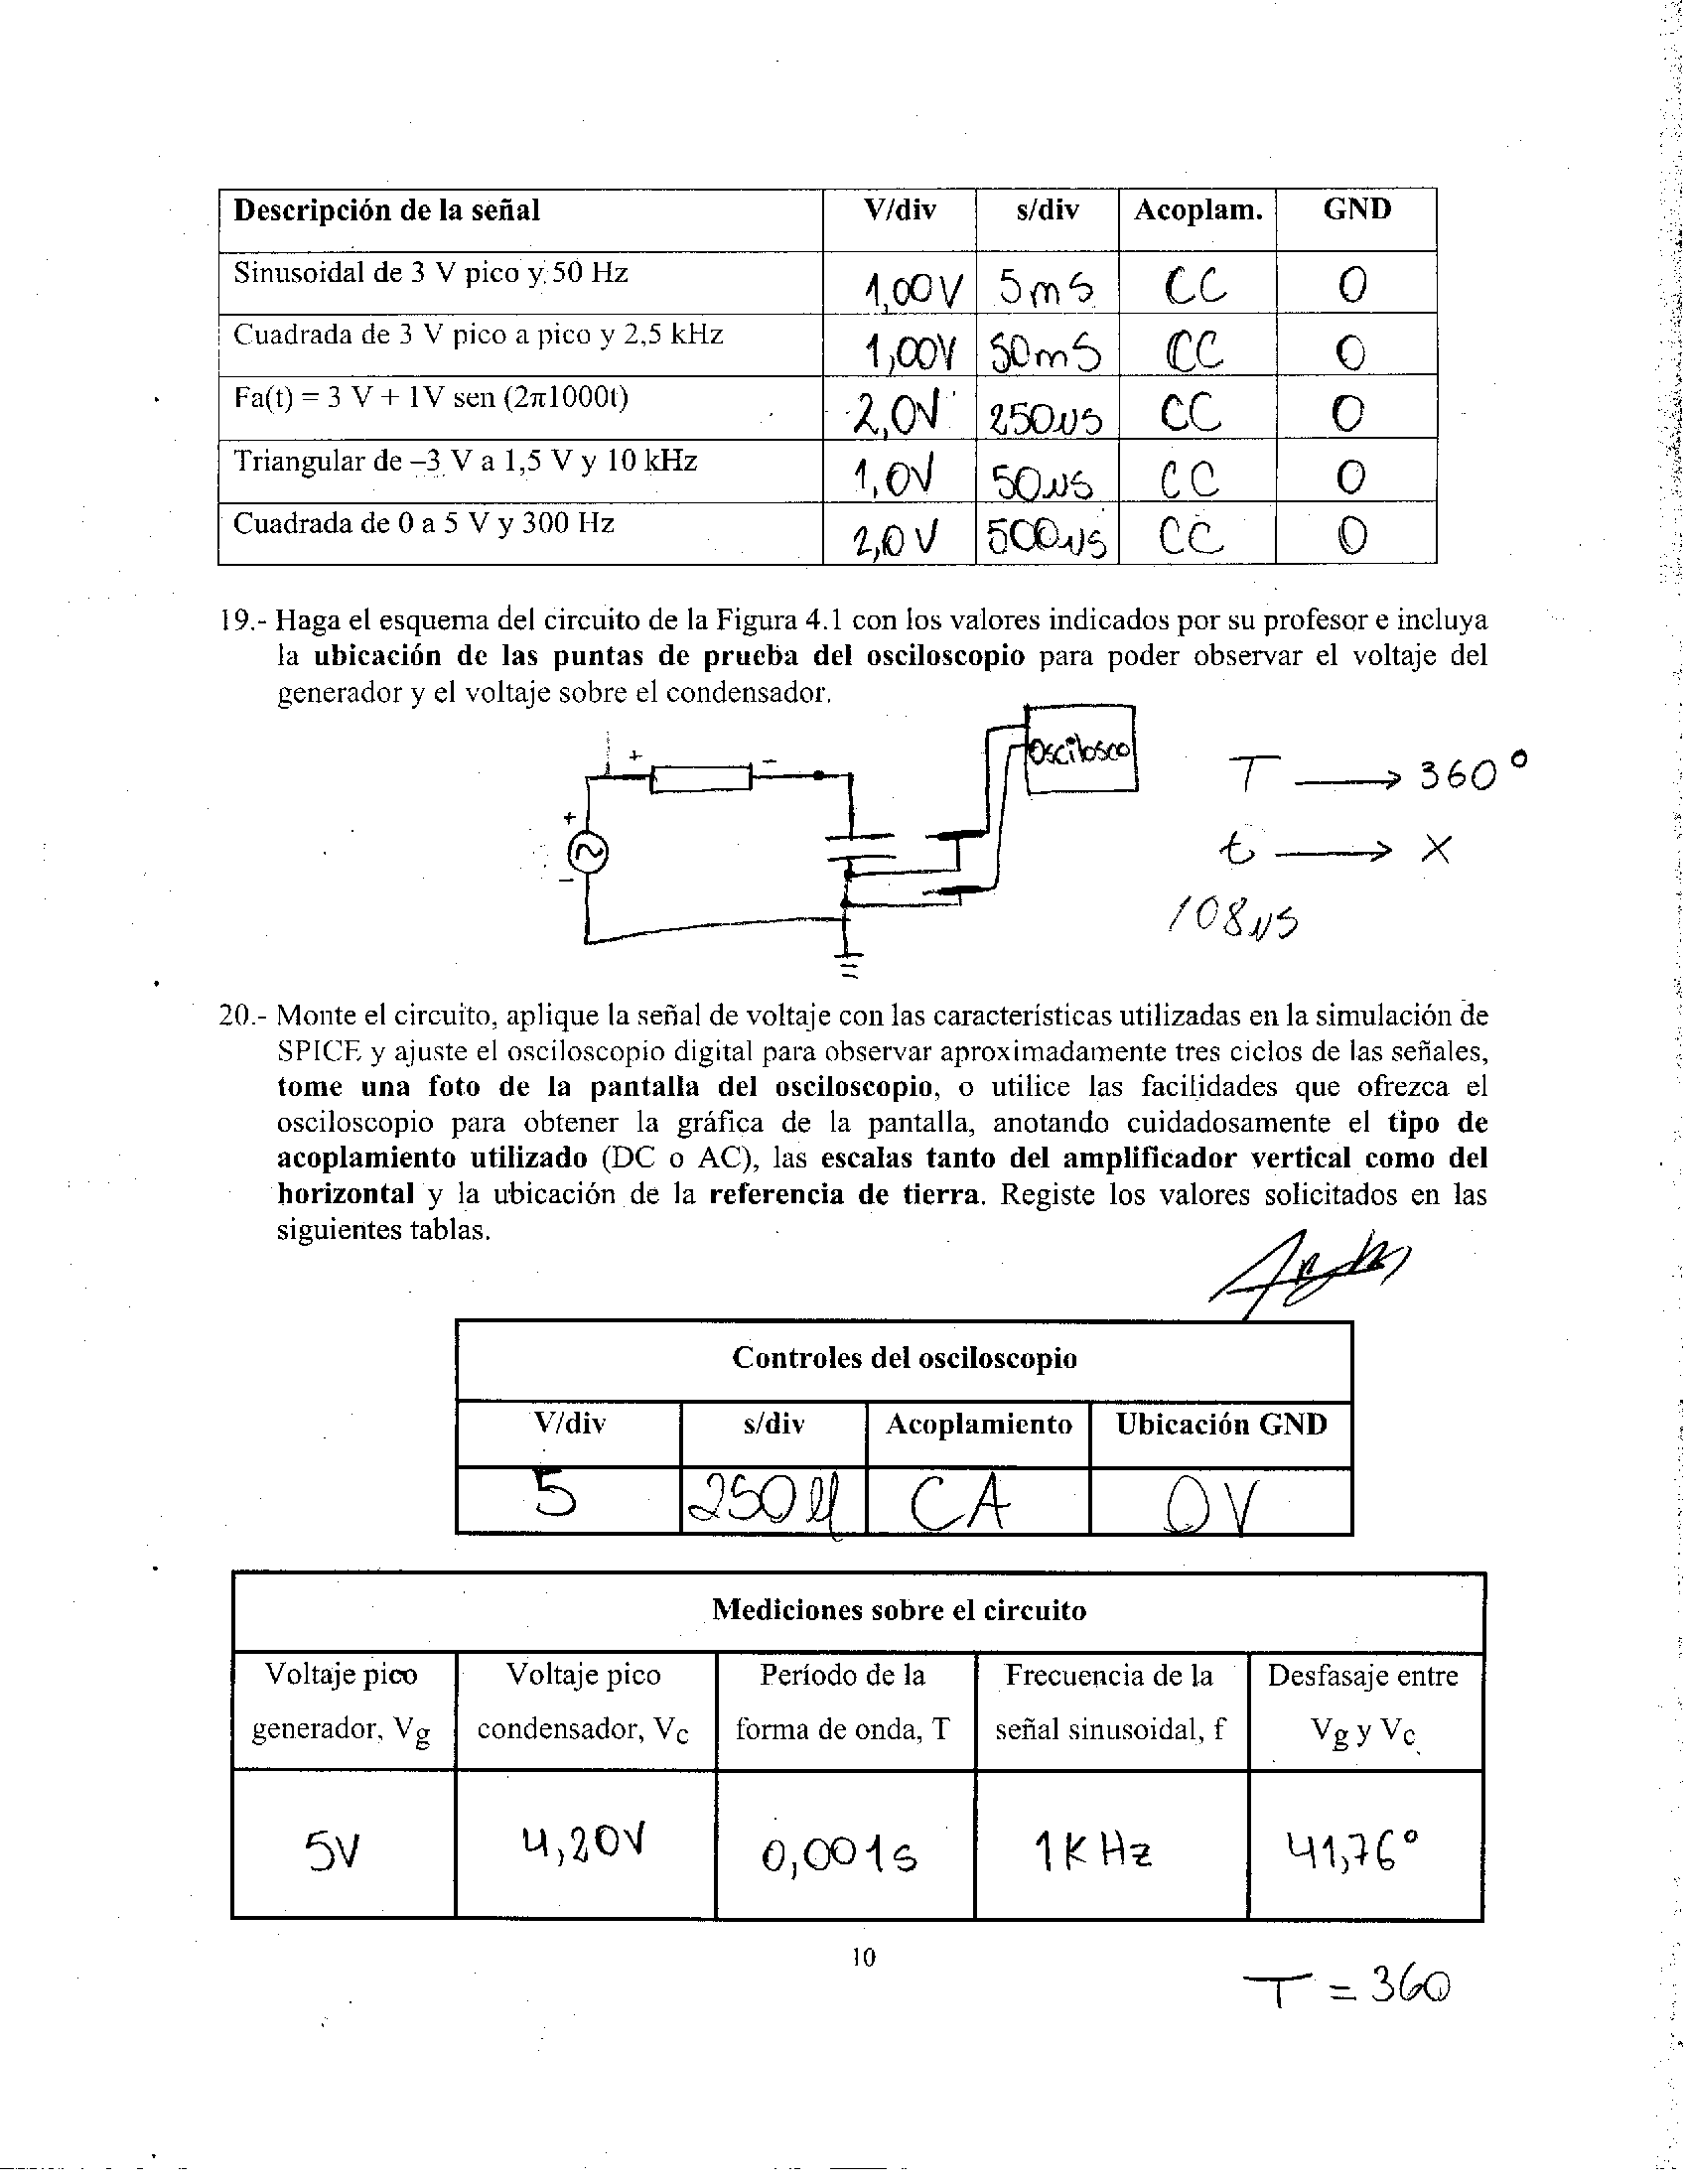
\includegraphics[width=16cm,height=20cm]{Img/anex_lab_4_0006}
	\end{center}
	
	\begin{center}
		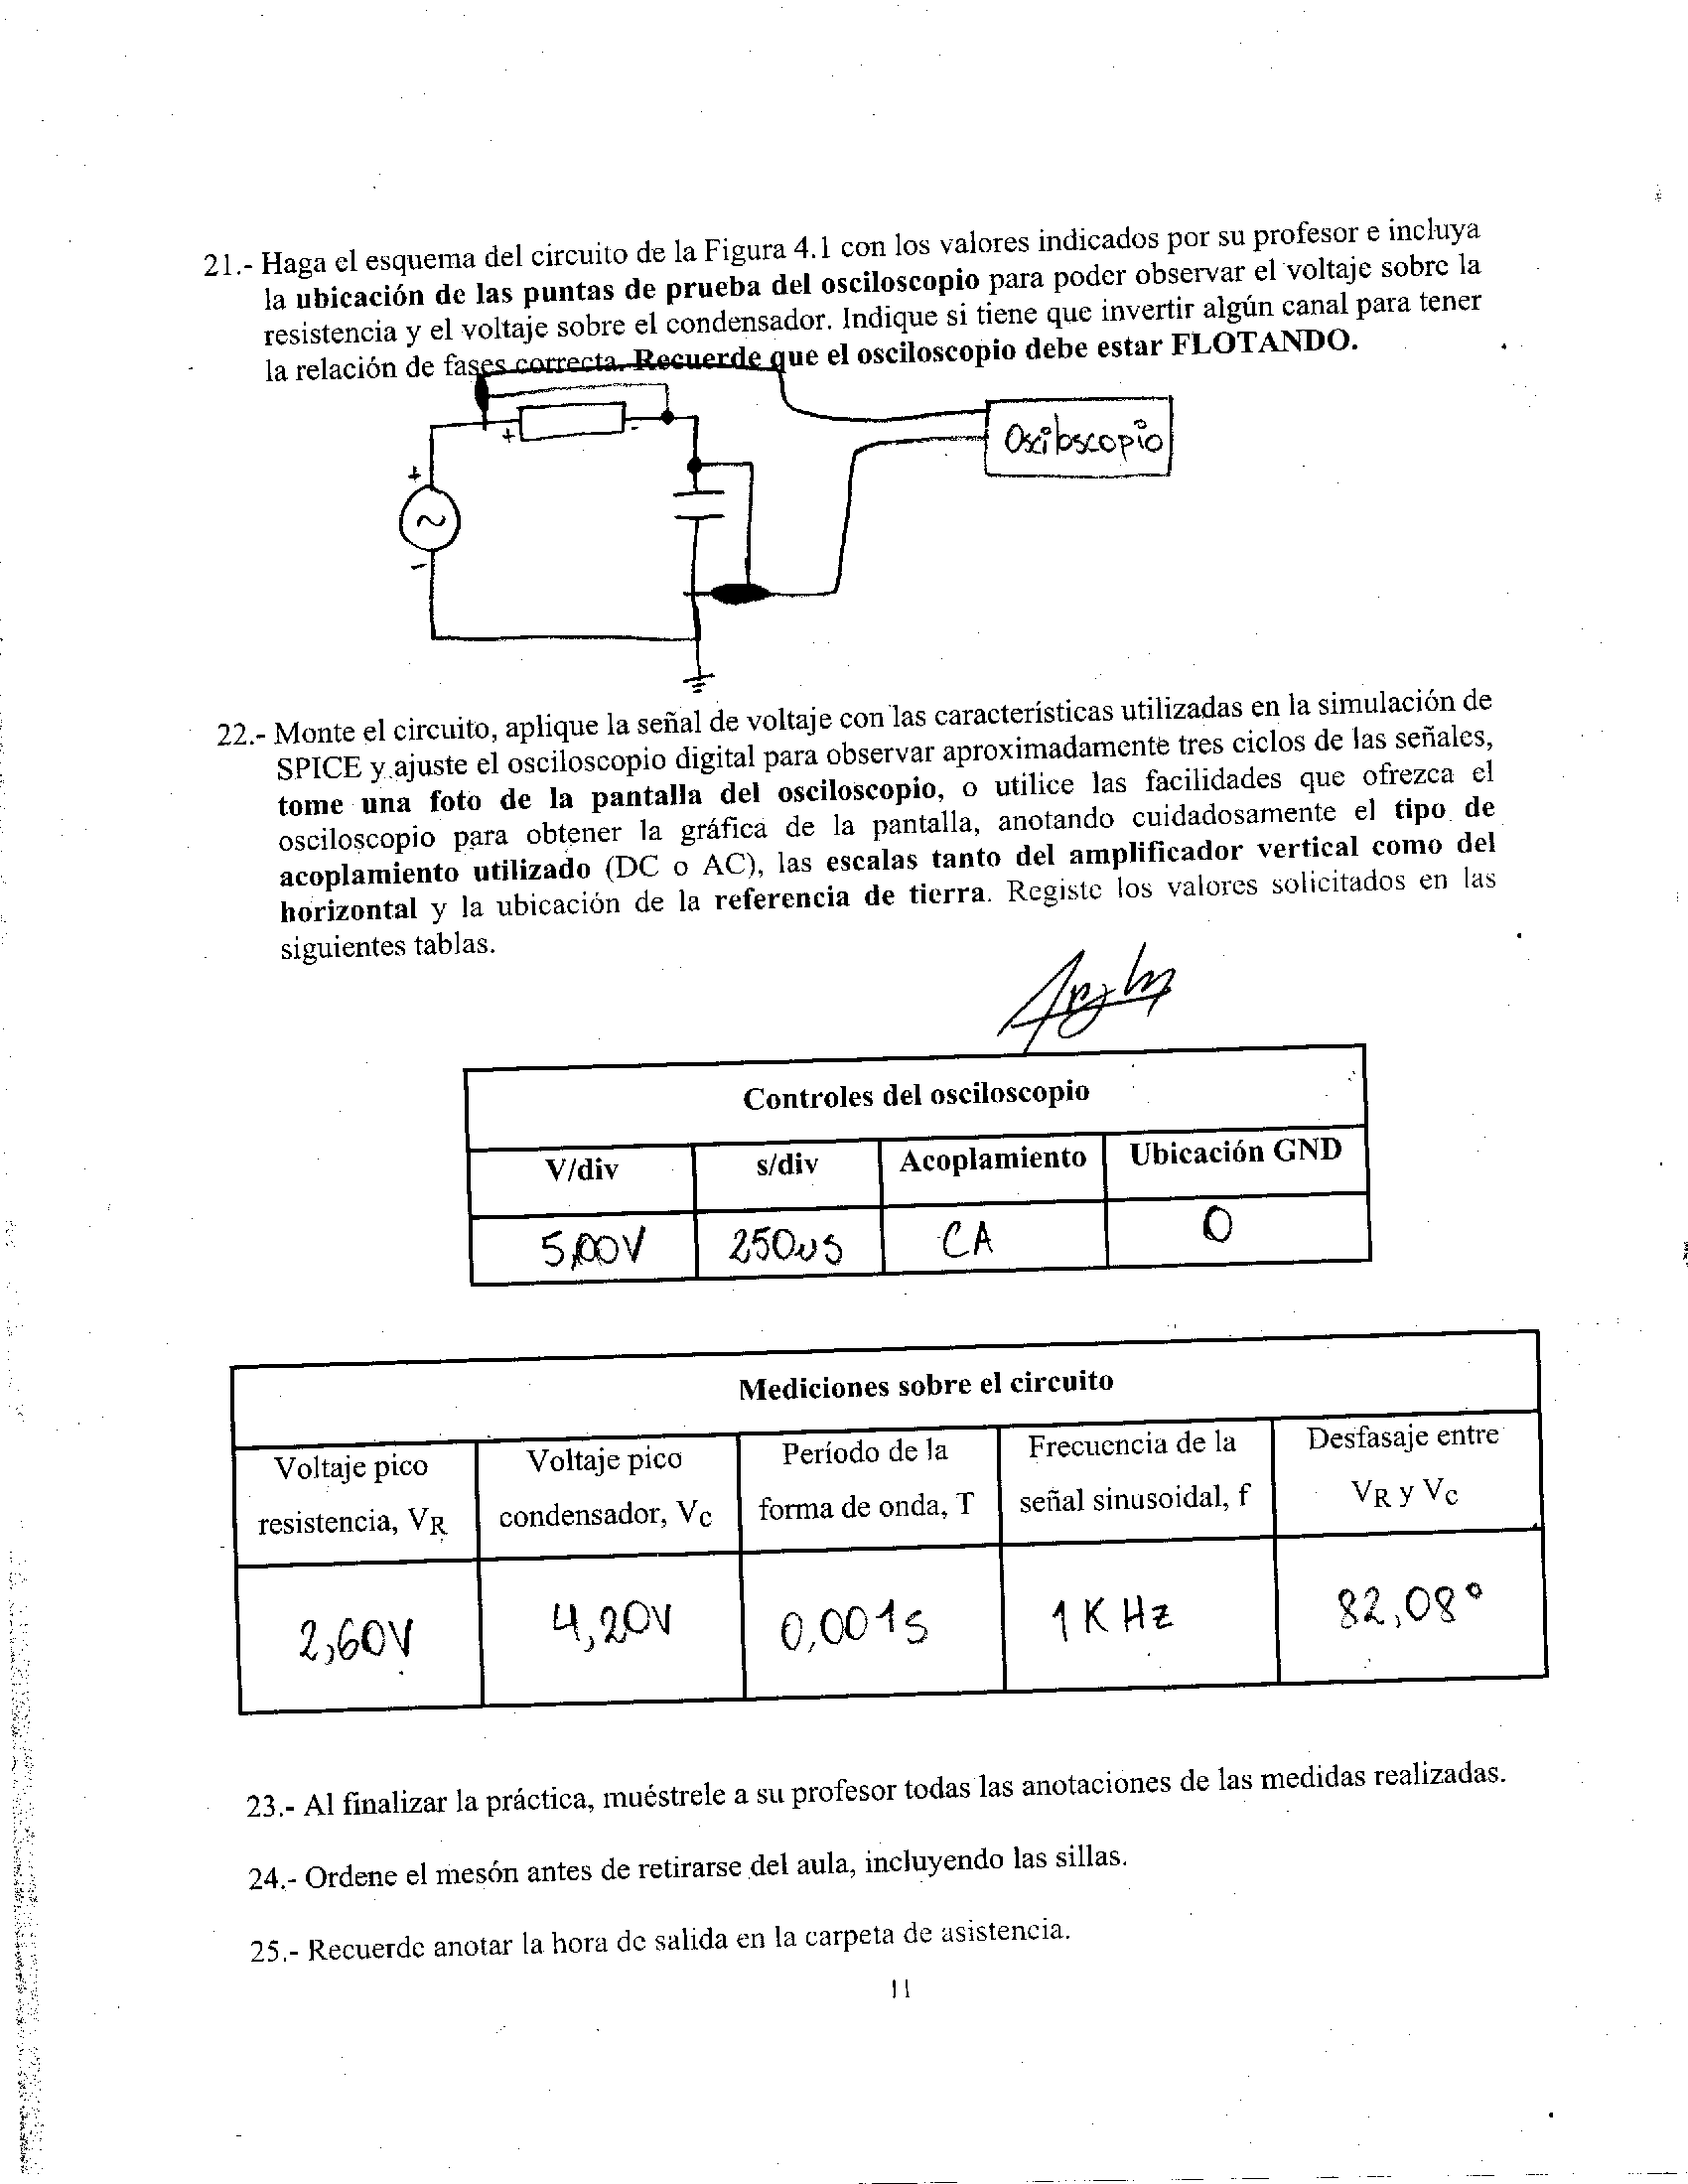
\includegraphics[width=16cm,height=20cm]{Img/anex_lab_4_0007}
	\end{center}
	
	
	\newpage
	
	\newpage
	
	\begin{center}
		\textbf{\large ANÁLISIS DE RESULTADOS}\\
	\end{center}
	
	\noindent Tiempo atrás durante la práctica de Spice, uno de los circuitos simulados concuerda con el que se estudió durante esta práctica, un circuito RC en corriente alterna, el circuito en cuestión seguía el siguiente esquema:
	
	\begin{center}
		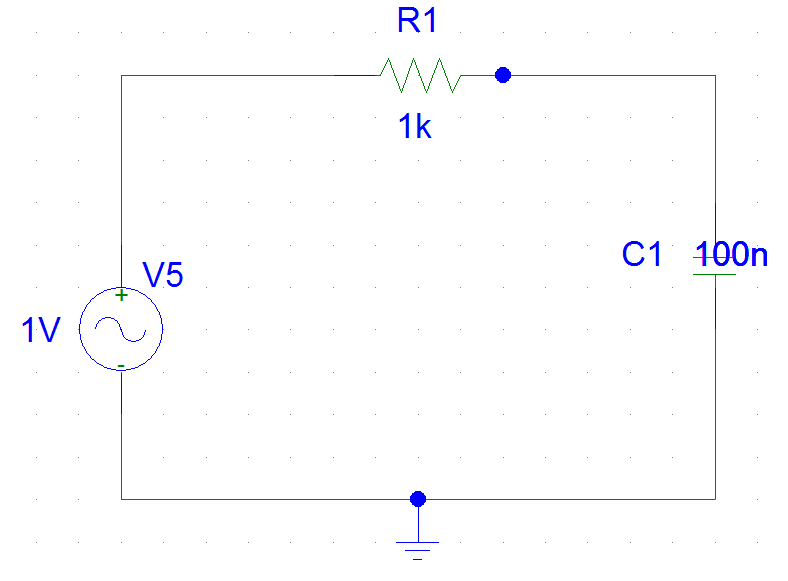
\includegraphics[width=10cm,height=8cm]{Img/ac_rc}
	\end{center}
	
	\noindent Al medir el voltaje de la fuente y en el capacitor para esa disposición se obtuvo el siguiente análisis:
	
	\begin{center}
		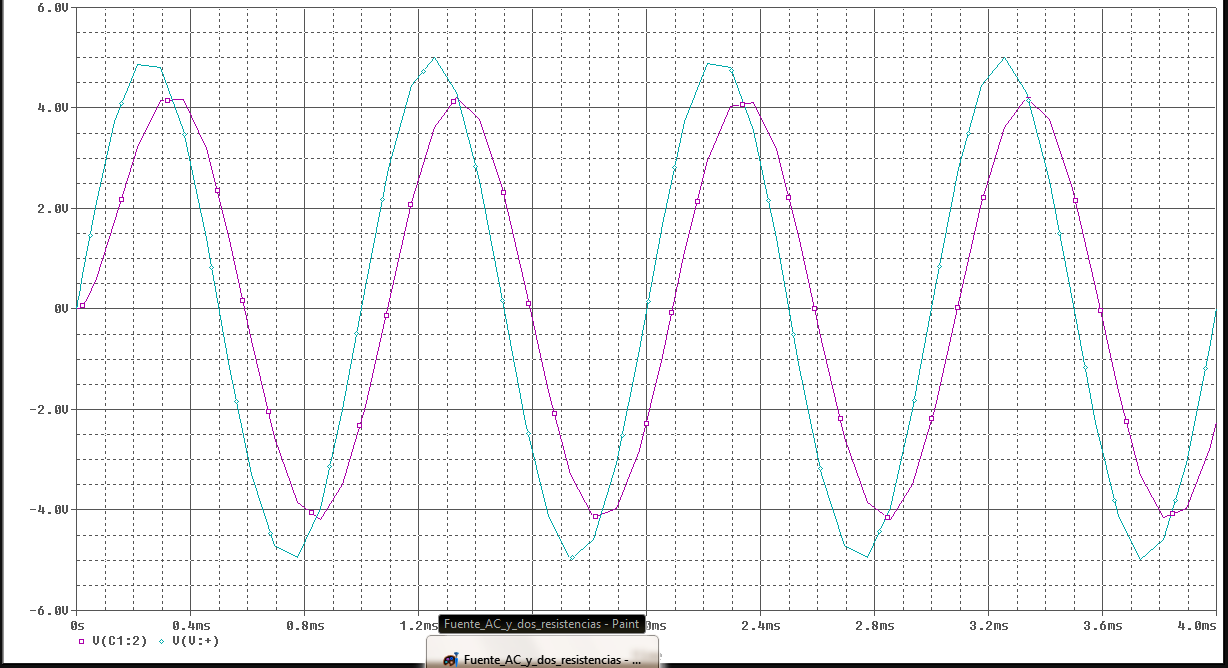
\includegraphics[width=10cm,height=8cm]{Img/fuente_capacitor_spice}
	\end{center}
	
	\newpage
	
	\noindent Luego al replicar ese circuito en el laboratorio se obtuvo:
	
	\begin{center}
		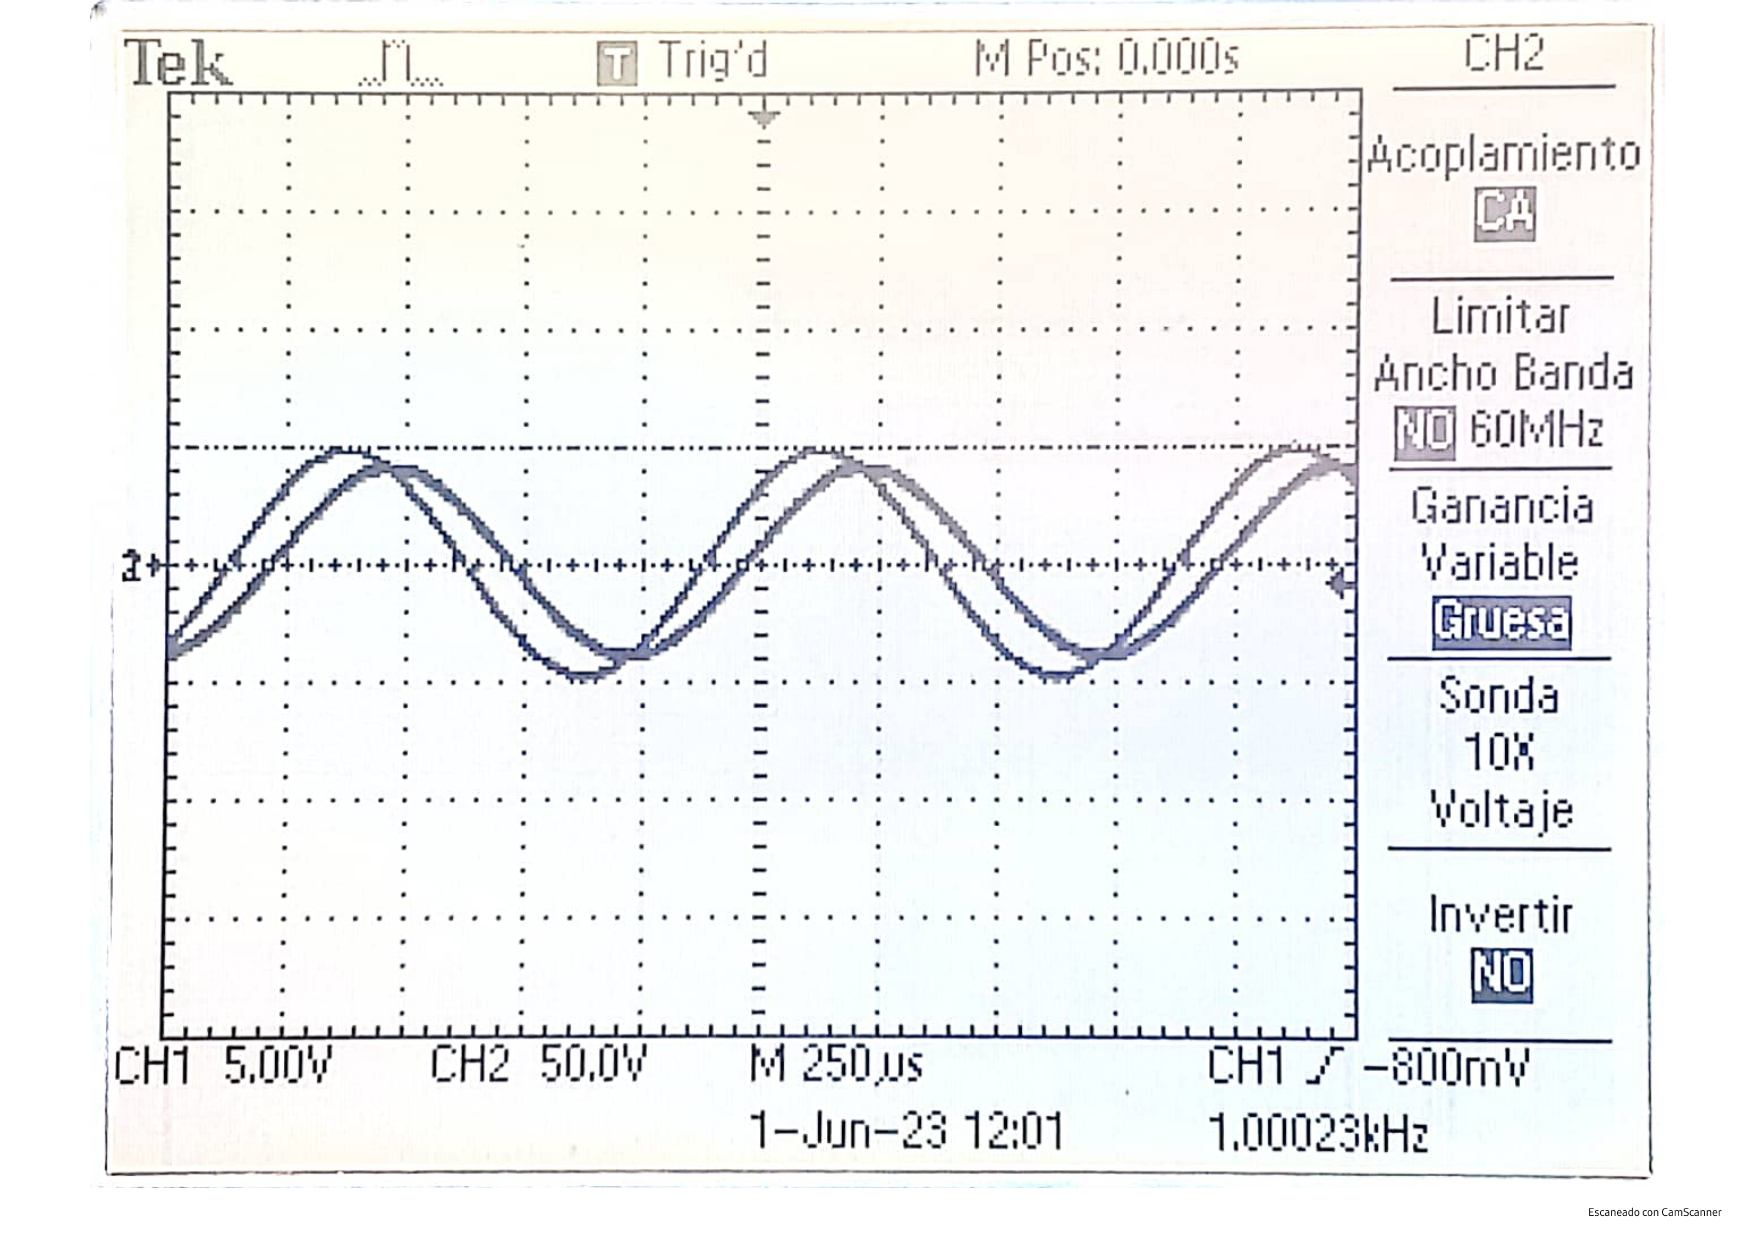
\includegraphics[width=10cm,height=8cm]{Img/fuente_capacitor}
	\end{center}
	
	\noindent Se puede apreciar que el defase del capacitor respecto a la fuente se mantiene igual como debería y que ambas gráficas son sumamente similares, las diferencias radican en detalles como la salida en el generador de ondas y la escala observada, sin embargo, las gráficas son perfectamente análogas.
	
	\noindent También tendremos que al medir el voltaje en la resistencia vs el voltaje en el capacitor en spice resultó en:
	
	\begin{center}
		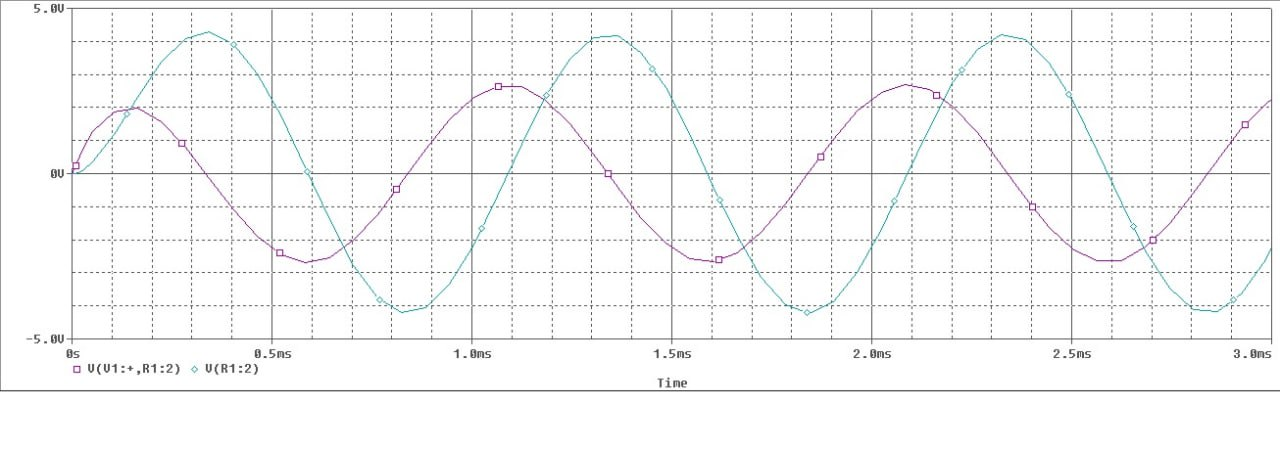
\includegraphics[width=10cm,height=8cm]{Img/capacitor_resistencia_spice}
	\end{center}
	
	\noindent En spice cambiar los elementos evaluados sólo implicaba, sin embargo en la práctica implicó cambiar las conexiones del osciloscopio e invertir la señal del capacitor ya que al ser medida por algunas carracterísticas del modo flotante, el voltaje medido en el capacitor tenía polaridad invertida, después de configurar todo, se obtuvo:
	
	\begin{center}
		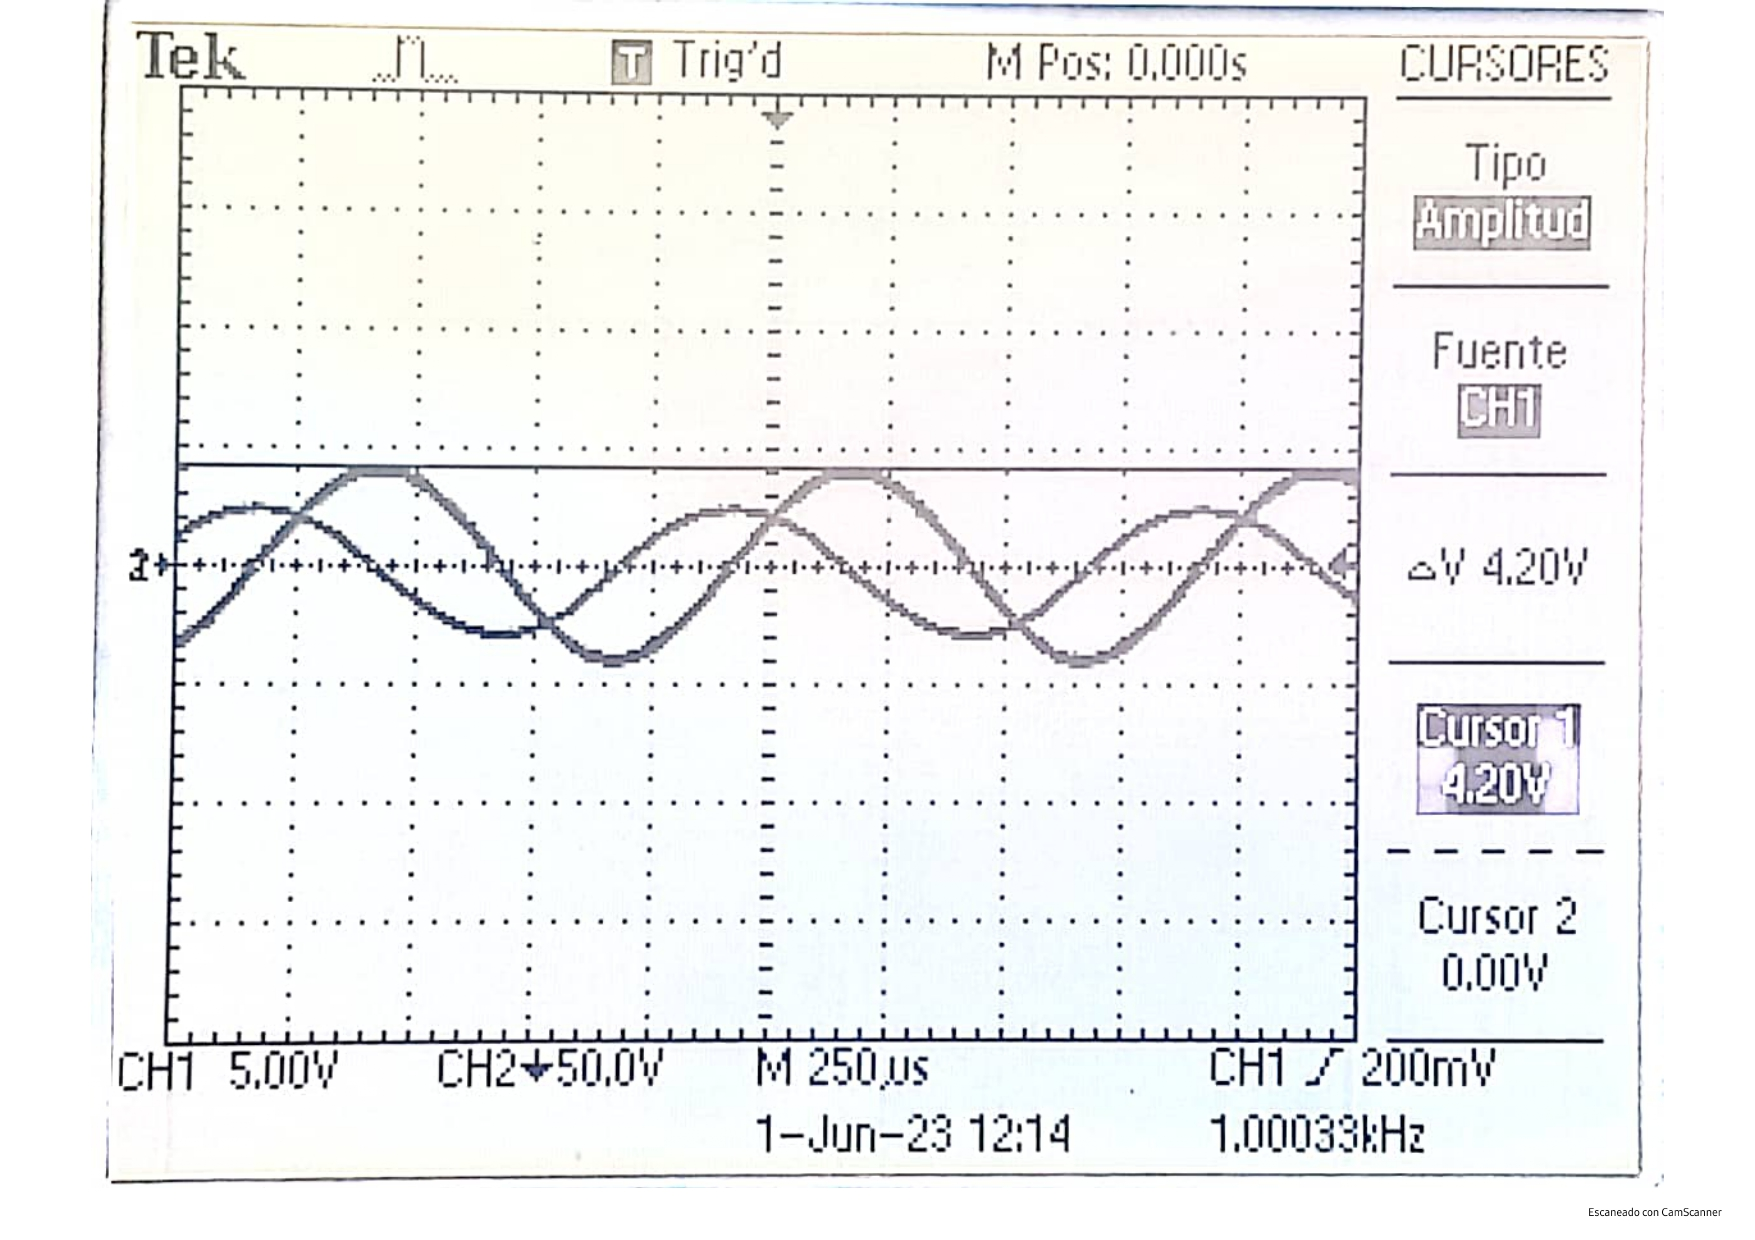
\includegraphics[width=10cm,height=8cm]{Img/capacitor_resistencia}
	\end{center}

	\noindent Como se puede apreciar, al igual que antes, la gráfica obtenida es análoga a la ue generó spice, confirmando así que lo planteado teóricamente se cumple al tener un circuito físico funcionando.\\
	
	\noindent Para ambos pares de gráficas destaca que cada par es análogo entre sí y ue las diferencias radican en las escalas del multímetro, el voltaje suministrado por el generador de fuentes y la configuracipon de la gráfica en spice, aún así, queda en evidencia que spice es una herramienta formidable para probar circuito antes de montarlos, lo que permite esstimar eficiencia, optimizar gastos y perfeccionar los circuitos.
	
	\newpage
	
	\begin{center}
		\textbf{\large CONCLUSIONES}\\
	\end{center}
	
	\renewcommand{\theenumi}{\alph{enumi}} %Letras minúsculas 
	
	\begin{enumerate}
		
		\item Precisión y exactitud de las medidas de voltaje DC
		tomadas con el osciloscopio:
		
		\noindent En cuanto a la precisión, el osciloscopio cuenta con $\frac{1}{5}$ del voltaje de la escala por división, así que sin los cursores, se tiene una precisión de hasta una unidad menos que la unidad mostrada, lo cual no es suficiente para medir decimales, pero permite llegar a un buen aproximado del voltaje medido.\\
		
		\noindent Para la exactitud se pudo apreciar que es sumamente formidable, ya que para cada función generada el valor mostrado en el osciloscopio era más exacto que el tomado con el multímetro.\\
		
		\begin{center}
			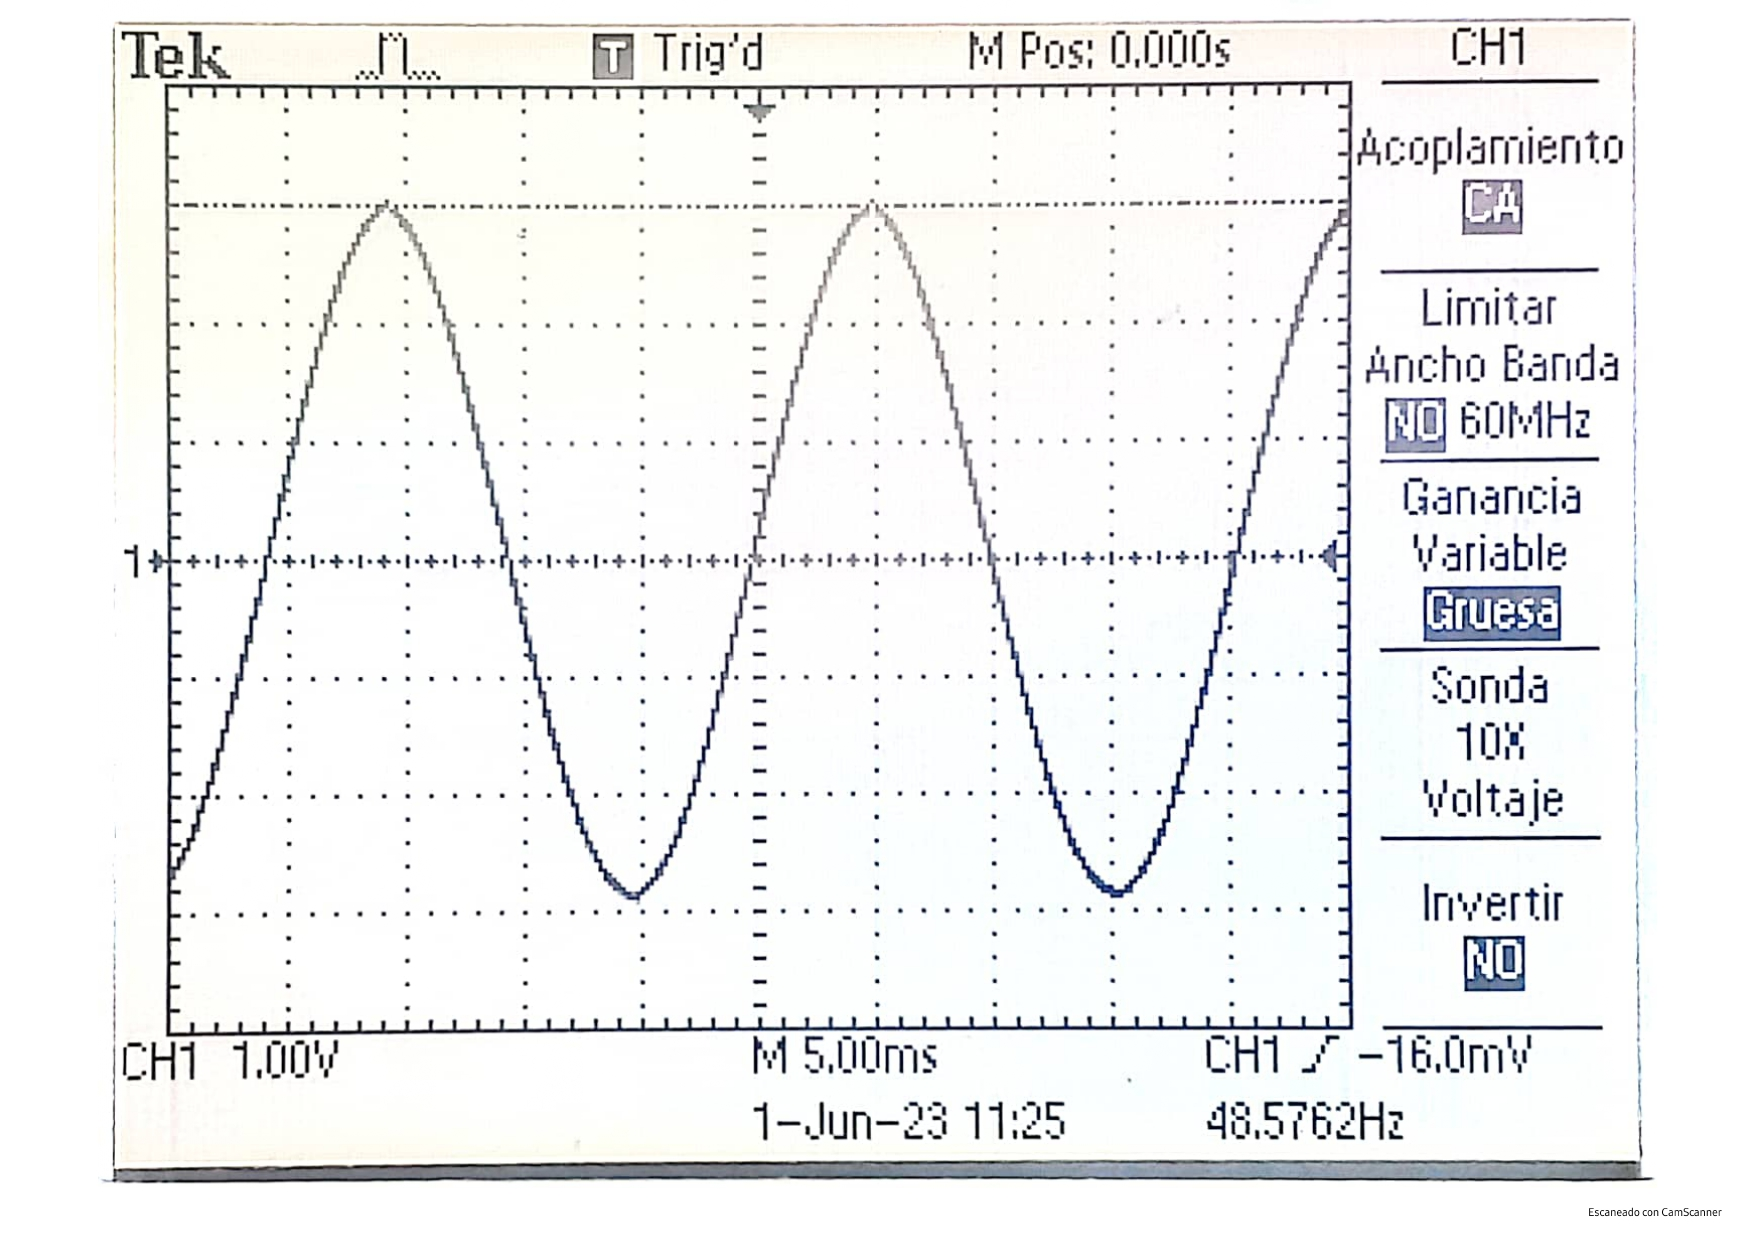
\includegraphics[width=10cm,height=8cm]{Img/medicion_sin_cursores}
		\end{center}
		
		\item Precisión de las medidas de voltaje AC tomadas por el osciloscopio usando cursores:
		
		\noindent Con los cursores la precisión del osciloscopio aumenta de manera considerable ya que se pueden usar para llegar a un mejor acercamiento respecto a los decimales, dando paso a medidas aún más precisas.
		
		\begin{center}
			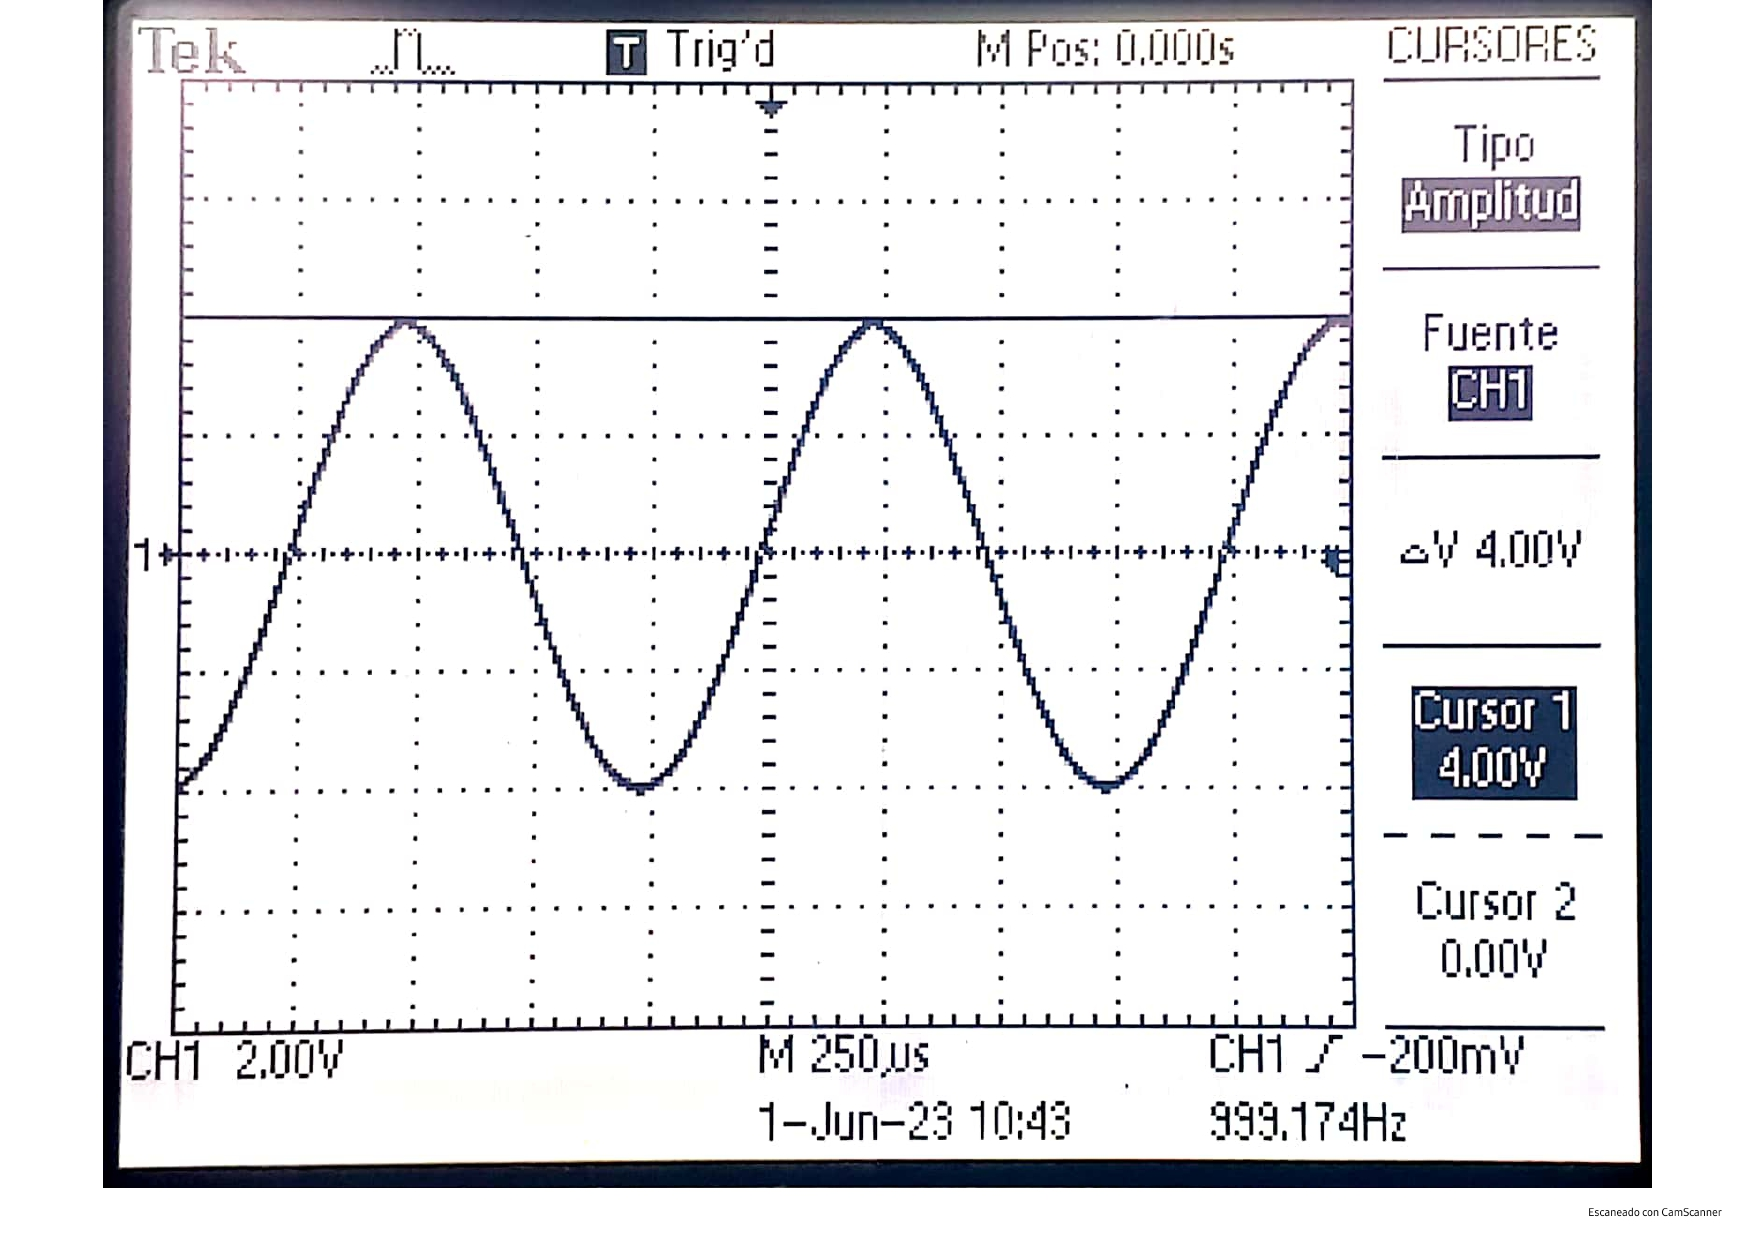
\includegraphics[width=10cm,height=8cm]{Img/medicion_cursores}
		\end{center}
		
		\item Precisión de las medidas de desfasaje
		tomadas con el osciloscopio:
		
		\noindent El desfasaje medido también tiene una precisión sumamente adecuada ya que al igual que con voltaje, el tiempo se mide con cada división y cada subdivisión representa $\frac{1}{5}$ de la escala de tiempo, además, al usar cursores se adquiere una precisión excelente.\\
		
		\item Utilidad de poder realizar mediciones con
		acoplamiento DC y AC:
		
		\noindent El acoplamiento DC detecta la señal y la posiciona con el voltaje de offset en caso de existir, mientras que el acoplamiento AC proporciona la señal eliminando cualquier offset.\\
		
		\noindent El primero nos permite evaluar la señal cuando se trabaja con un offset y así poder examinar los valores reales.
		
		\begin{center}
			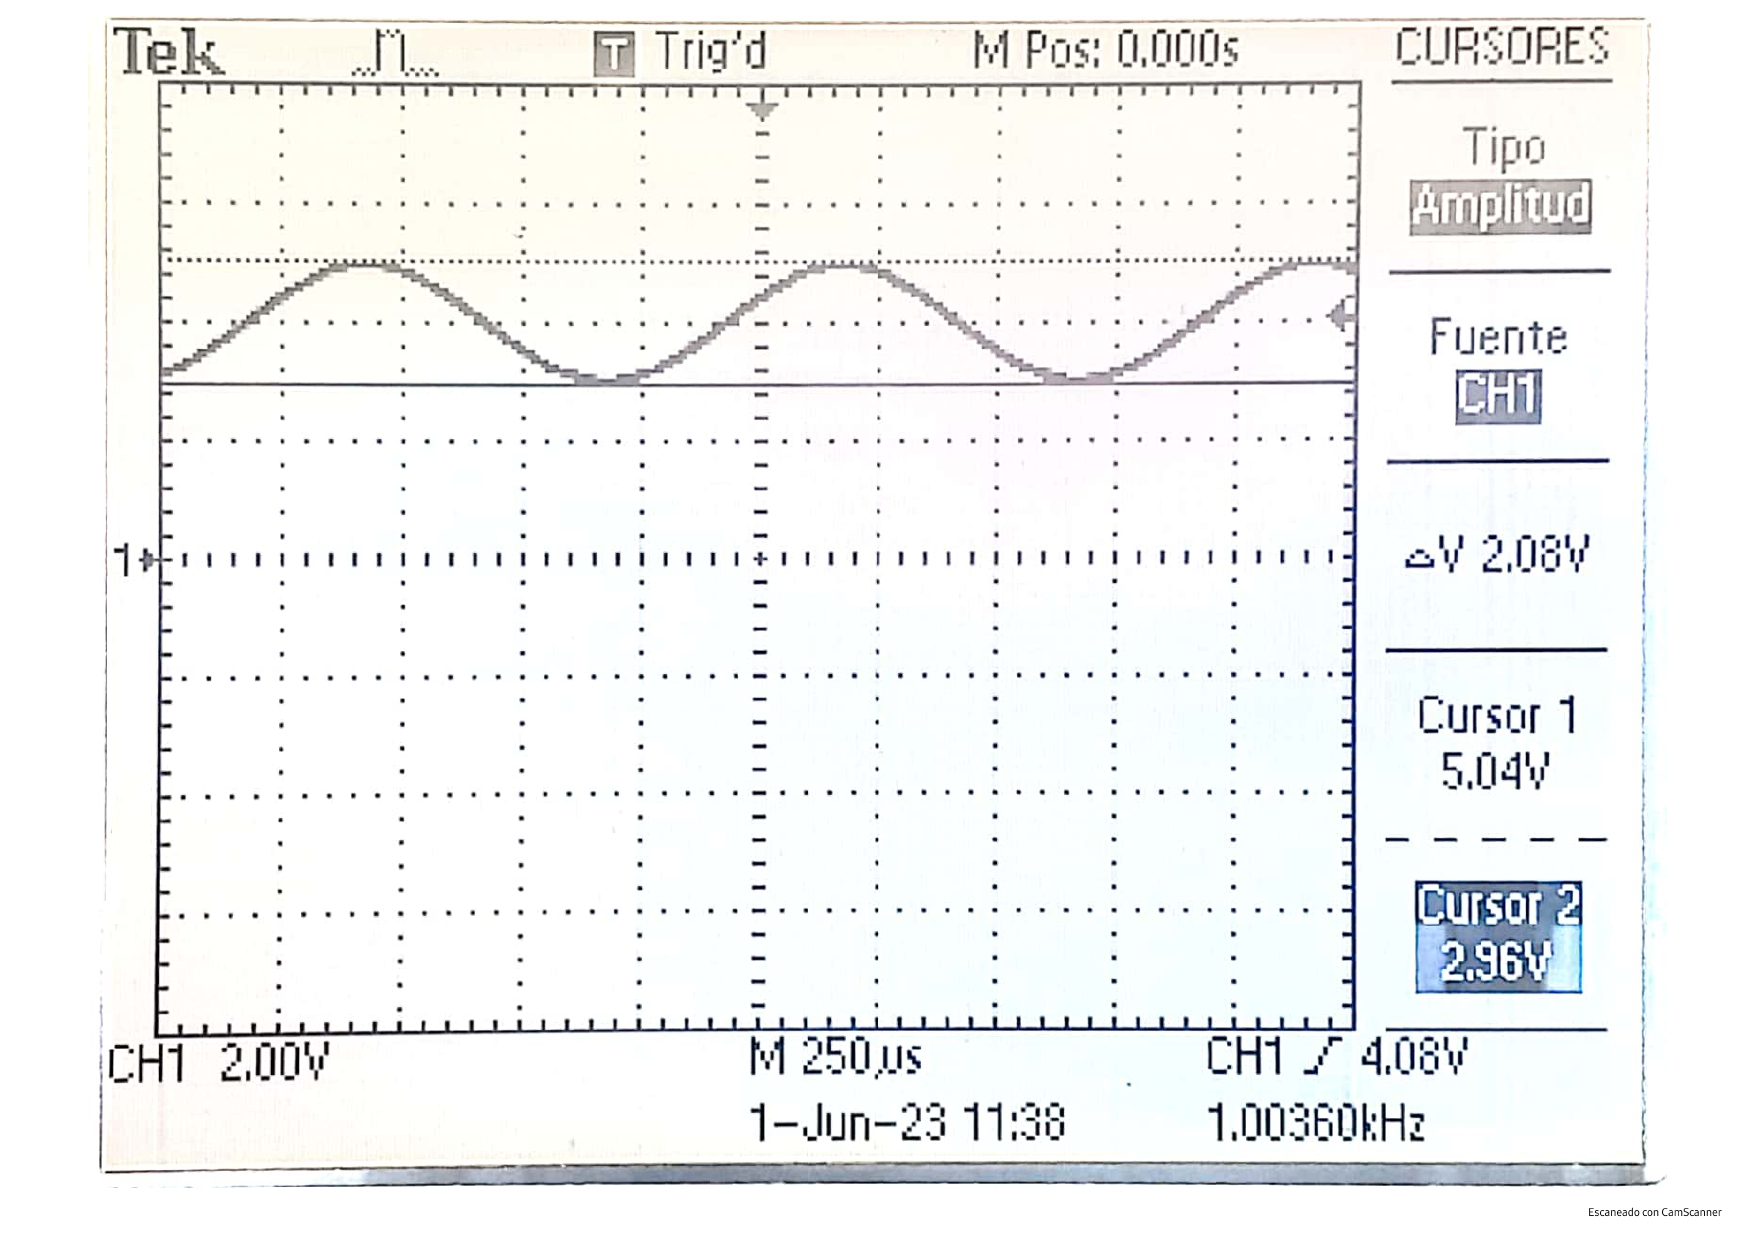
\includegraphics[width=10cm,height=8cm]{Img/con_offset}
		\end{center}
	
		\noindent El acople AC no permite que pase ningún offset, lo cual ess sumamente útil si se tiene un voltaje con offset y se quiere estudiar la señal senoidal pura evitando que se aleje del centro.\\
		
		\item Conclusiones generales:
		
		\noindent El osciloscopio llegó para revolucionar el dominio humano sobre la electricidad, permitiendo caracterizar y estudiar a fondo las señales.\\
		
		\noindent Esta herramienta es la base de sistemas eléctricos complejos y electrónica de potencia ya que permite visualizar las señales sinusoidales para realizar diseños complejos.\\
		
		\noindent Comparar señales, estudiar amplitudes, frecuencias, etc, son cosas que sin el osciloscopio serían imposibles. A su vez tenemos el osciloscopio analógico que fue el precursor de toda esta tecnología y el digital que facilita procesos y provee de una mayor gama de opciones.\\
		
		\noindent El osciloscopio es sin duda una herramienta indispensable en el mundo moderno.
		
	\end{enumerate}
	
	\newpage
	
	\begin{center}
		\textbf{\large BIBLIOGRAFÍA}\\
	\end{center}
	
	\noindent Laboratorios de Circuitos Electrónicos, Guía Teórica versión electrónica, ubicada en la página web del laboratorio C, http://www.labc.usb.ve, enlace a "Páginas web de Asignaturas", EC1281-Laboratorio de Mediciones Eléctricas 2013.
	
\end{document}

